\documentclass[11pt,a4paper]{article}

% ------------------------------------------------------------------
% Packages
% ------------------------------------------------------------------
\usepackage[utf8]{inputenc}
\usepackage[T1]{fontenc}
\usepackage{lmodern}
\usepackage{amsmath,amssymb,amsthm,mathtools}
\usepackage{bm}
\usepackage[margin=2.7cm]{geometry}
\usepackage{enumitem}
\usepackage[colorlinks=true,linkcolor=blue!50!black,citecolor=blue!50!black,urlcolor=blue!50!black]{hyperref}
\usepackage[capitalise,noabbrev]{cleveref}
\usepackage{xcolor}
\usepackage{graphicx}
\usepackage{booktabs}

% ------------------------------------------------------------------
% Theorem environments
% ------------------------------------------------------------------
\theoremstyle{plain}
\newtheorem{theorem}{Theorem}[section]
\newtheorem{proposition}[theorem]{Proposition}
\newtheorem{lemma}[theorem]{Lemma}
\newtheorem{corollary}[theorem]{Corollary}
\theoremstyle{definition}
\newtheorem{definition}[theorem]{Definition}
\newtheorem{assumption}[theorem]{Assumption}
\newtheorem{example}[theorem]{Example}
\theoremstyle{remark}
\newtheorem{remark}[theorem]{Remark}

% ------------------------------------------------------------------
% Macros
% ------------------------------------------------------------------
\newcommand{\E}{\mathbb{E}}
\newcommand{\Prob}{\mathbb{P}}
\newcommand{\1}{\mathbf{1}}
\newcommand{\F}{\mathcal{F}}
\newcommand{\R}{\mathbb{R}}
\newcommand{\Var}{\operatorname{Var}}
\newcommand{\Cov}{\operatorname{Cov}}
\newcommand{\infconv}{\mathbin{\square}}
\crefname{assumption}{Assumption}{Assumptions}
\crefname{remark}{Remark}{Remarks}
\crefname{definition}{Definition}{Definitions}
\crefname{example}{Example}{Examples}
\crefname{figure}{Figure}{Figures}
\crefname{table}{Table}{Tables}

\title{Pricing Parlays by Hedging on Prediction-Market Order Books}
\author{}
\date{\today}

\begin{document}
\maketitle

\begin{abstract}
A bookmaker without a view on outcomes can set the odd of a bet by the cost of hedging it on a prediction market, where each event trades as a binary contract through an order book. For a single event the hedge is static and exact. For a parlay on several events decided at the same time, with no market on their joint outcome, we show that every static hedge, and every dynamic hedge required to be safe on every path, costs at least the upper Fréchet bound: the odd it supports is that of the least likely leg alone, and a parlay quoted at that odd is dominated by single bets. We therefore study dynamic hedges that accept a controlled error. An exact product identity yields a hedge in closed form: each leg is held in proportion to the fair value of the parlay on the other legs. Under the assumptions that fair values are martingales and that legs are conditionally independent, this hedge is variance-optimal, and its error has a policy-independent floor that vanishes as rebalancing becomes frequent. We show that zero expected error is a property of the capital charged, not of the strategy, and decompose the error of any strategy into capital, deviation and covariation terms. With order books, we bound the friction cost of rebalancing, analyse no-trade bands, and derive the quoted odd as the solution of a fixed-point equation that interpolates between the static odd and the competitive parlay odd. Extensions to dependent legs and to $n$ legs, and a simulation of two football matches, illustrate the results.
\end{abstract}

% ==================================================================
\section{Introduction}
\label{sec:intro}
% ==================================================================

\paragraph{The problem.}
A \emph{parlay} (or accumulator) is a single bet on the joint occurrence of several events, called its \emph{legs}. Let $S>0$ denote the bettor's stake and $o\geq 1$ the (decimal) \emph{odd} quoted by the bookmaker, that is, the amount paid back per unit staked if the bet wins. The bettor receives $S\,o$ if \emph{all} legs win, and nothing otherwise. We study how a bookmaker should quote $o$ when it has no opinion of its own on the outcomes. Its only information, and its only means of laying off risk, is a prediction market \cite{WolfersZitzewitz2004} on which each individual event is traded as a binary contract paying $1$ if the event occurs and $0$ otherwise.

The guiding principle is that the \emph{odd is determined by the cost of hedging}. Let $m\in[0,1)$ denote the bookmaker's margin, the fraction of the stake it keeps, and let $N := S\,o$ denote the payout promised to the bettor. The bookmaker spends the remaining $S(1-m)$ on a trading strategy in the prediction market whose terminal value covers $N$ whenever the bet wins. The odd offered is the largest one for which this is possible, under a criterion to be made precise. Prices therefore come from the market, not from a forecasting model, and the bookmaker's profit comes from the margin, not from outcome risk.

\paragraph{The single-event benchmark.}
For a single event the principle gives a complete answer. The prediction market does not offer a single price but an order book, a ladder of resting offers at increasing prices. Let $p(q)$ denote the average execution price obtained when buying $q$ contracts by walking this ladder, and let $c(q) := q\,p(q)$ denote the resulting total cost; $c$ is piecewise linear, increasing and convex. Since each contract pays $1$, holding $q$ contracts pays $q$ if the event occurs. A static purchase of $N$ contracts therefore pays exactly $N$ when the bet wins, so the hedge is exact, model-free and executed once. The payout that can be hedged is the number of contracts the net stake buys. Since $c$ is strictly increasing, it is invertible, and this number is
\[
N(S) := c^{-1}\bigl(S(1-m)\bigr).
\]
Let $\bar p(S) := S(1-m)/N(S) = p\bigl(N(S)\bigr)$ denote the average price paid for these contracts. The odd is then
\[
o(S) = \frac{N(S)}{S} = \frac{1-m}{\bar p(S)}.
\]
The odd depends on the stake: because $c$ is convex, the average price $\bar p(S)$ is non-decreasing in $S$, so larger bets receive lower odds. This is the market odd net of margin and price impact: safe on every path and commercially competitive.

\paragraph{The difficulty with parlays.}
Consider now a two-leg parlay on events $A$ and $B$. For an event $E$, let $\1_E$ denote its indicator, equal to $1$ if $E$ occurs and $0$ otherwise. The bookmaker's \emph{liability}, the amount it owes the bettor at settlement, is then $N\,\1_{A\cap B}$. Three features of the setting make the problem non-trivial.
\begin{enumerate}[label=(\roman*)]
  \item \emph{No joint market.} Only the marginal contracts $\1_A$ and $\1_B$ are traded. If a contract on $A\cap B$ were listed, the single-event argument would apply verbatim with its order book.
  \item \emph{Simultaneous events.} The two events are decided over the same time window, so the bookmaker cannot hedge sequentially by rolling the proceeds of the first leg into the second.
  \item \emph{Order books, not prices.} At every time the cost of trading depends on direction and size; there is no single tradable price, and every rebalancing is costly.
\end{enumerate}
The natural first attempt is a static portfolio of the two marginal contracts, bought once and held to settlement. Let $p_A$ and $p_B$ denote the prices of the contracts on $A$ and $B$, ignoring price impact for this discussion; they can be read as market-implied probabilities of the two events. The cheapest static portfolio that is safe in every outcome costs $N\min(p_A,p_B)$. This equals $N$ times the upper Fréchet bound $\min(p_A,p_B)$, the largest value $\Prob(A\cap B)$ can take among all joint distributions $\Prob$ with marginal probabilities $p_A$ and $p_B$. The resulting odd is the odd of the less likely leg alone: the bettor bears the risk of the second leg and is paid nothing for it. Static hedging is therefore safe but commercially useless, and any competitive quote must use the fact that the order books keep trading while the events are live.

\paragraph{Contributions.}
The paper makes the following contributions.
\begin{enumerate}[label=(\arabic*)]
  \item \emph{Static impossibility.} We formulate static hedging as a linear programme and show by duality that its value is exactly the Fréchet bound $N\min(p_A,p_B)$. Price impact, represented by the infimal convolution of the leg cost functions, can only raise this cost.
  \item \emph{A variance-optimal dynamic hedge in closed form.} Let $t_0<t_1<\dots<t_K$ denote the rebalancing times. At each time $t_k$, let $m^A_k$ and $m^B_k$ denote the \emph{fair values} of the two contracts, estimates of the events' probabilities lying within the bid--ask spread, and let $q^A_k$ and $q^B_k$ denote the numbers of contracts held. Under the assumptions that fair values are martingales (the formal meaning of ``no view'') and that the legs are conditionally independent, an exact discrete product identity yields the hedge $q^A_k = N m^B_k$, $q^B_k = N m^A_k$, with initial capital $N p_A p_B$. The trade in each leg equals $N$ times the change in the \emph{other} leg's fair value. The hedge is valid for jumps of any size, and we prove it is variance-optimal.
  \item \emph{A decomposition of hedging error valid for every policy.} The hedge error of any strategy splits into a capital term, a deviation-from-target term and a covariation term. We show that zero expected error is a property of the capital charged, not of the strategy, and that the strategy determines only the variance. That variance has a policy-independent floor, plus a quadratic penalty for deviating from the target.
  \item \emph{Friction costs.} With order books, rebalancing costs spread and impact. We obtain closed-form upper bounds on expected impact costs and a lower bound on spread costs in terms of the legs' probabilities, and we analyse no-trade band policies that trade cost against variance.
  \item \emph{An odds-setting rule.} Combining these results gives a fixed-point equation for the offered odd. Its solution interpolates between the competitive parlay odd $(1-m)/(p_A p_B)$ when books are deep and the static odd $(1-m)/\min(p_A,p_B)$ when books are thin.
\end{enumerate}
We are also explicit about what dynamic hedging cannot achieve. If safety on every path is required, the hedging cost reverts to the static Fréchet bound, so any quote better than the static one rests on a dependence assumption between the legs. The approach turns that assumption into a covariation risk which is measurable in real time and can be reserved for.

\paragraph{Outline.}
\Cref{sec:setup} introduces the notation, the order-book cost functions and the notion of hedging cost. \Cref{sec:single} treats the single-event bet. \Cref{sec:static} proves the static impossibility result for two-leg parlays. \Cref{sec:dynamic} develops the frictionless dynamic hedge and the error decomposition, and \cref{sec:frictions} adds spread and price impact. \Cref{sec:odds} turns hedging cost into an odd. \Cref{sec:robust} discusses correlation, worst-case hedging and practical risks. \Cref{sec:nlegs} extends the construction to $n$ legs, \cref{sec:numerics} gives a numerical illustration, and \cref{sec:conclusion} concludes.

% ==================================================================
\section{Setup and notation}
\label{sec:setup}
% ==================================================================
This section fixes the notation used throughout the paper. The definitions given informally in \cref{sec:intro} are restated here formally, so that the technical development does not depend on the introduction.

\subsection{The bet}

\begin{definition}[Bet]
\label{def:bet}
A \emph{bet} is described by the following quantities:
\begin{itemize}
  \item the \emph{stake} $S>0$, paid by the bettor to the bookmaker when the bet is placed;
  \item the \emph{margin} $m\in[0,1)$, the fraction of the stake the bookmaker keeps as compensation and does not invest in the hedge;
  \item the \emph{odd} $o\geq 1$, quoted by the bookmaker in decimal form;
  \item the \emph{payout} $N := S\,o$, paid by the bookmaker to the bettor if the bet wins.
\end{itemize}
The \emph{net stake} $S(1-m)$ is the amount available to the bookmaker to finance the hedge.
\end{definition}

Only the payout $N$ enters the hedging problem; the stake, margin and odd enter only through the relation between the cost of the hedge and the net stake (\cref{def:quote} below). We assume a zero interest rate throughout; funding costs are introduced in \cref{sec:odds}.

\subsection{Events, information and time}

Let $(\Omega,\F,\Prob)$ be a probability space, where $\Prob$ is the real-world probability measure. The bookmaker does not know $\Prob$; it is used only to state which outcomes are possible (statements holding $\Prob$-almost surely) and, from \cref{sec:dynamic} onwards, to state the modelling assumptions under which the dynamic results hold.

Let $A,B\in\F$ denote the events on which the parlay is written, called its \emph{legs}. For an event $E\in\F$, the \emph{indicator} $\1_E:\Omega\to\{0,1\}$ equals $1$ on $E$ and $0$ on its complement $E^c$. We assume that all four \emph{joint outcomes}
\[
A\cap B,\qquad A\cap B^c,\qquad A^c\cap B,\qquad A^c\cap B^c
\]
have positive probability; otherwise the parlay degenerates to a bet on a single event.

Let $T>0$ denote the \emph{settlement time}, by which both events are decided. Trading is allowed at the \emph{trading times}
\[
0 = t_0 < t_1 < \dots < t_{K-1} < t_K = T,
\]
with $K\geq 1$; at $t_K=T$ the contracts settle and no further trading takes place. Information is described by a filtration $(\F_k)_{k=0}^{K}$, where $\F_k\subseteq\F$ represents everything observable at time $t_k$: the state of both games and both order books. We assume that $\1_A$ and $\1_B$ are $\F_K$-measurable, that is, both outcomes are known at settlement. The case $K=1$, with a single trading time, is the \emph{static} case of \cref{sec:single,sec:static}.

\subsection{Binary contracts}

For each leg $E\in\{A,B\}$, the prediction market lists a \emph{binary contract} on $E$, which pays $\1_E$ at time $T$: one unit of cash per contract if $E$ occurs and nothing otherwise. Holding $q$ contracts therefore pays $q\,\1_E$ at settlement.

\begin{assumption}[Frictionless settlement]
\label{ass:settlement}
Settlement is free: a contract held until time $T$ pays exactly $\1_E$, without fees or the need to trade.
\end{assumption}

As a consequence, costs arise only from trading, never from holding a position until settlement. In particular, a position need not be unwound before $T$.

\begin{assumption}[Short positions]
\label{ass:short}
A negative holding $q<0$ is allowed and pays $q\,\1_E$ at settlement.
\end{assumption}

\Cref{ass:short} is consistent with how binary prediction markets operate. Such markets usually list a complementary contract paying $\1_{E^c} = 1-\1_E$, so a short position of $|q|$ contracts on $E$ is equivalent to holding $|q|$ complementary contracts together with a cash liability of $|q|$. We work with signed holdings in the contract on $E$ only, and assume that the bid side of its order book (defined next) already accounts for any liquidity available through the complementary contract.

\subsection{The order book as a cost function}

At each trading time, the order book of a contract consists of resting offers to sell (the \emph{ask side}) and resting offers to buy (the \emph{bid side}).

\begin{definition}[Order book]
\label{def:book}
An \emph{order book} consists of
\begin{itemize}
  \item ask levels $(\alpha_j,s_j)_{j=1}^{J}$, where $\alpha_j\in(0,1)$ is the price of the $j$-th offer to sell, $s_j>0$ its size in contracts, and $\alpha_1<\alpha_2<\dots<\alpha_J$;
  \item bid levels $(\beta_j,r_j)_{j=1}^{J'}$, where $\beta_j\in(0,1)$ is the price of the $j$-th offer to buy, $r_j>0$ its size in contracts, and $\beta_1>\beta_2>\dots>\beta_{J'}$;
\end{itemize}
satisfying $\beta_1\leq\alpha_1$. We call $\alpha_1$ the \emph{best ask}, $\beta_1$ the \emph{best bid}, and
\[
D^{\mathrm{ask}} := \sum_{j=1}^{J} s_j,\qquad D^{\mathrm{bid}} := \sum_{j=1}^{J'} r_j
\]
the \emph{depths} of the two sides.
\end{definition}

The requirement that all prices lie strictly between $0$ and $1$ excludes offers that would be arbitrages against settlement, since a contract never pays more than $1$ or less than $0$.

A trade of size $\delta\in\R$ means buying $\delta$ contracts if $\delta>0$ and selling $|\delta|$ contracts if $\delta<0$. A trade is executed by consuming the best available levels first.

\begin{definition}[Cost function]
\label{def:cost}
The \emph{cost function} of an order book is the map $c$ from $[-D^{\mathrm{bid}},D^{\mathrm{ask}}]$ to $\R$ giving the cash paid for a trade of size $\delta$:
\[
c(\delta) :=
\begin{cases}
\displaystyle\sum_{j=1}^{J} \alpha_j \min\Bigl\{s_j,\ \bigl(\delta - \textstyle\sum_{i<j}s_i\bigr)^+\Bigr\}, & \delta\geq 0,\\[3ex]
\displaystyle-\sum_{j=1}^{J'} \beta_j \min\Bigl\{r_j,\ \bigl(|\delta| - \textstyle\sum_{i<j}r_i\bigr)^+\Bigr\}, & \delta<0,
\end{cases}
\]
where $x^+ := \max\{x,0\}$. A negative value $c(\delta)<0$ means cash is received.
\end{definition}

The cash received when selling $q>0$ contracts is $-c(-q)$. For $q\neq 0$, the \emph{average execution price} of a trade of size $q$ is
\[
p(q) := \frac{c(q)}{q}.
\]
This extends the function $p$ of \cref{sec:intro}, which was defined only for purchases. For $q>0$, $p(q)$ is the average price paid when buying; for $q<0$, it is the average price received when selling.

\begin{lemma}[Properties of the cost function]
\label{lem:cost}
The cost function $c$ of \cref{def:cost} has the following properties.
\begin{enumerate}[label=(\alph*)]
  \item $c(0)=0$.
  \item $c$ is continuous, piecewise linear and strictly increasing.
  \item $c$ is convex.
  \item The subdifferential of $c$ at $0$ is the bid--ask interval: $\partial c(0) = [\beta_1,\alpha_1]$.
  \item $p$ is non-decreasing on $(0,D^{\mathrm{ask}}]$ and on $[-D^{\mathrm{bid}},0)$, with $p(q)\leq\beta_1\leq\alpha_1\leq p(q')$ for all $q<0<q'$.
\end{enumerate}
\end{lemma}

\begin{proof}
Property (a) is immediate. On the buy side, $c$ is linear with slope $\alpha_j$ on the interval $\bigl[\sum_{i<j}s_i,\ \sum_{i\leq j}s_i\bigr]$; on the sell side, it is linear with slope $\beta_j$ on $\bigl[-\sum_{i\leq j}r_i,\ -\sum_{i<j}r_i\bigr]$. This gives continuity and piecewise linearity, and all slopes are positive, which gives (b). Reading from left to right, the slopes are $\beta_{J'}<\dots<\beta_1\leq\alpha_1<\dots<\alpha_J$, a non-decreasing sequence; a continuous piecewise linear function with non-decreasing slopes is convex, which gives (c). The left and right derivatives at $0$ are $\beta_1$ and $\alpha_1$, which gives (d). For (e), $p(q) = (c(q)-c(0))/(q-0)$ is the slope of the chord of $c$ from $0$ to $q$; by convexity this slope is non-decreasing in $q$ on each side of $0$, and lies below the left derivative $\beta_1$ for $q<0$ and above the right derivative $\alpha_1$ for $q>0$.
\end{proof}

Property (e) states the two forms of price impact: larger purchases are made at higher average prices, larger sales at lower average prices, and every round trip loses at least the spread $\alpha_1-\beta_1$.

The order book changes over time. For each leg $E\in\{A,B\}$ and trading time $t_k$, let $c^E_k$ denote the cost function of the order book of the contract on $E$ at time $t_k$, with depths $D^{\mathrm{ask},E}_k$ and $D^{\mathrm{bid},E}_k$, best ask $\alpha^E_{1,k}$ and best bid $\beta^E_{1,k}$. The book at $t_k$ is observable at $t_k$, so $c^E_k$ is $\F_k$-measurable.

\begin{assumption}[No persistent impact]
\label{ass:impact}
The order books $(c^E_k)_{k}$ are exogenous: the bookmaker's trades at time $t_k$ consume liquidity in the book at $t_k$, but do not affect the books at later trading times.
\end{assumption}

\Cref{ass:impact} is the standard simplification that the book fully replenishes between trading times. It is reasonable when the bookmaker's trades are small relative to the flow of orders between trading times, and it keeps the cost of a strategy additive over time.

\subsection{Trading strategies}

\begin{definition}[Strategy]
\label{def:strategy}
A \emph{strategy} with \emph{initial capital} $x_0\in\R$ is a sequence of holdings $(q^A_k,q^B_k)_{k=0}^{K-1}$, where $q^E_k$ is the number of contracts on $E$ held after trading at $t_k$ and kept until $t_{k+1}$. The holdings must satisfy:
\begin{itemize}
  \item \emph{adaptedness}: $q^A_k$ and $q^B_k$ are $\F_k$-measurable, so decisions use only information available at $t_k$;
  \item \emph{feasibility}: setting $q^E_{-1}:=0$, the trade $\delta^E_k := q^E_k - q^E_{k-1}$ lies in $\bigl[-D^{\mathrm{bid},E}_k,\ D^{\mathrm{ask},E}_k\bigr]$, so it can be executed against the book at $t_k$.
\end{itemize}
\end{definition}

For $k=0,\dots,K$, let $x_k$ denote the \emph{cash account} just before trading at $t_k$, equivalently the cash held over the period $(t_{k-1},t_k]$; at $k=K$ it is the cash held at settlement. The bookmaker starts with cash $x_0$ and no contracts. Each trade is paid for in cash at the price given by the current order book, and cash earns no interest, so the cash account evolves as
\[
x_{k+1} = x_k - c^A_k\bigl(\delta^A_k\bigr) - c^B_k\bigl(\delta^B_k\bigr),\qquad k=0,\dots,K-1.
\]
Over the period $(t_k,t_{k+1}]$ the bookmaker therefore holds the cash $x_{k+1}$ together with the contracts $q^A_k$ and $q^B_k$. Iterating the recursion gives the cash account explicitly:
\[
x_k = x_0 - \sum_{j=0}^{k-1}\Bigl(c^A_j\bigl(\delta^A_j\bigr) + c^B_j\bigl(\delta^B_j\bigr)\Bigr),\qquad k=0,\dots,K,
\]
with the empty sum equal to $0$ for $k=0$. The cash account may become negative, which corresponds to borrowing at zero interest. By \cref{ass:settlement}, the value of the portfolio at settlement is
\[
X_T := x_K + q^A_{K-1}\,\1_A + q^B_{K-1}\,\1_B.
\]

\begin{definition}[Hedge error]
\label{def:error}
Let $N\geq 0$ be the payout of a parlay on $A$ and $B$. The \emph{liability} is the random variable $H := N\,\1_{A\cap B}$, and the \emph{hedge error} of a strategy is
\[
\mathcal{E} := X_T - H.
\]
The event $\{\mathcal{E}<0\}$ is a \emph{shortfall}: the portfolio does not cover the amount owed, and the bookmaker must cover the difference $-\mathcal{E}$ from its own funds.
\end{definition}

\subsection{Hedging cost and quoted odds}

Whether a strategy is good enough is decided by a criterion on its hedge error. We formalise this as a set of acceptable errors, and keep the criterion general at this stage.

\begin{definition}[Acceptance set]
\label{def:acceptance}
An \emph{acceptance set} $\mathcal{A}$ is a set of random variables, interpreted as the hedge errors the bookmaker is willing to bear.
\end{definition}

Two acceptance sets will be used in the paper:
\begin{itemize}
  \item the \emph{superhedging} set $\mathcal{A}^{\mathrm{sup}} := \{\mathcal{E}:\ \mathcal{E}\geq 0\ \Prob\text{-a.s.}\}$, which accepts only strategies that cover the liability in every possible outcome;
  \item sets defined by the mean and dispersion of $\mathcal{E}$, which accept a shortfall in some outcomes provided its expectation and risk are controlled; these are made precise in \cref{sec:dynamic,sec:odds}.
\end{itemize}
The set $\mathcal{A}^{\mathrm{sup}}$ requires no knowledge of $\Prob$ beyond which outcomes are possible, which is the sense in which superhedging is model-free.

\begin{definition}[Hedging cost]
\label{def:hedgecost}
Given an acceptance set $\mathcal{A}$, the \emph{hedging cost} of the payout $N$ is
\[
C_{\mathcal{A}}(N) := \inf\bigl\{x_0\in\R:\ \text{some strategy with initial capital } x_0 \text{ has hedge error in } \mathcal{A}\bigr\},
\]
with the convention $\inf\emptyset = +\infty$.
\end{definition}

The hedging cost is the smallest amount of cash that, invested in the prediction market, produces an acceptable hedge of the liability. It is $+\infty$ when no feasible strategy is acceptable, for instance when the order books are too shallow to hedge the payout.

\begin{definition}[Quoted odd]
\label{def:quote}
Let $\mathcal{A}$ be an acceptance set, $m$ the margin and $S$ the stake. Of the stake received from the bettor, the bookmaker pockets $mS$ as its margin, and the remainder is the only cash it invests in the hedge. The initial capital of the hedging strategy is therefore the net stake,
\[
x_0 = S(1-m).
\]
The \emph{quoted odd} is the largest odd whose payout can be hedged acceptably starting from this capital:
\[
o_{\mathcal{A}}(S) := \sup\bigl\{o\geq 1:\ C_{\mathcal{A}}(S\,o)\leq x_0\bigr\} = \sup\bigl\{o\geq 1:\ C_{\mathcal{A}}(S\,o)\leq S(1-m)\bigr\}.
\]
In words, an odd $o$ can be offered only if the cheapest acceptable hedge of the promised payout $N=S\,o$ costs no more than the cash the bettor provides net of the margin. If no odd $o\geq 1$ satisfies this condition, the bookmaker declines the bet.
\end{definition}

The bookmaker's profit and loss on the bet thus splits into two parts: the margin $mS$, which is kept with certainty, and the hedge error $\mathcal{E}$ of a strategy started from $x_0 = S(1-m)$, which is acceptable by construction. The bookmaker takes no position on the outcome beyond what $\mathcal{A}$ tolerates.

\begin{remark}[Attainment]
\label{rem:attainment}
Since $C_{\mathcal{A}}$ is defined as an infimum, $C_{\mathcal{A}}(S\,o)\leq x_0$ does not by itself guarantee that an acceptable strategy starts from exactly $x_0$. Two conditions together ensure that it does. First, the acceptance set is \emph{monotone}: if $\mathcal{E}\in\mathcal{A}$ and $\mathcal{E}'\geq\mathcal{E}$, then $\mathcal{E}'\in\mathcal{A}$. Under this condition, unused cash only increases the hedge error, so a strategy that is acceptable from capital $x<x_0$ remains acceptable from $x_0$. Second, the infimum is attained when $C_{\mathcal{A}}(S\,o)=x_0$. Both conditions hold for $\mathcal{A}^{\mathrm{sup}}$ (attainment is shown in \cref{sec:single,sec:static}). For the acceptance sets introduced in later sections, we verify them or state explicitly where they fail.
\end{remark}

\Cref{def:quote} is the formal version of the guiding principle of \cref{sec:intro}: the odd is set by the cost of hedging, and the bookmaker earns the margin $mS$. \Cref{sec:single} shows that, for a single event under $\mathcal{A}^{\mathrm{sup}}$, the definition recovers the odd $o(S) = (1-m)/\bar p(S)$ derived in the introduction. The rest of the paper computes $C_{\mathcal{A}}$ for parlays under different choices of $\mathcal{A}$.

% ==================================================================
\section{Single-event bet}
\label{sec:single}
% ==================================================================
This section treats a bet on a single event, which serves as the benchmark for parlays. We show that buying the payout in contracts at the initial time and holding them to settlement is the cheapest hedge that is safe in every outcome, even when dynamic trading is allowed, and we derive the resulting odd.

\subsection{Specialisation of the setup}

A \emph{single-event bet} on $A$ pays $N = S\,o$ if $A$ occurs and nothing otherwise, so its liability is
\[
H := N\,\1_A.
\]
All definitions of \cref{sec:setup} apply with this liability in place of $N\,\1_{A\cap B}$ and with strategies that trade only the contract on $A$, that is, $q^B_k = 0$ for all $k$. To lighten notation in this section, we drop the superscript $A$ and write $c_k$, $q_k$, $\delta_k$ and $D^{\mathrm{ask}}_k$, $D^{\mathrm{bid}}_k$ for the cost function, holding, trade and depths of the contract on $A$ at time $t_k$. We work with the superhedging acceptance set $\mathcal{A}^{\mathrm{sup}}$ and write $C(N) := C_{\mathcal{A}^{\mathrm{sup}}}(N)$. By the standing assumption of \cref{sec:setup} that all joint outcomes have positive probability, both $\Prob(A)>0$ and $\Prob(A^c)>0$.

We also assume that the initial time carries no randomness: $\F_0$ is trivial, so the initial order book $c_0$ and the initial holding $q_0$ are deterministic. This holds because $t_0$ is the moment the bet is placed and the current book is observed.

\subsection{Cash as a substitute for contracts}

Beyond the depth of the ask side, the order book offers no more contracts, but the bookmaker can still cover a payout with cash: one unit of cash held to settlement pays $1$ whether or not $A$ occurs, which is at least what one contract pays. This motivates the following extension of the cost function.

\begin{definition}[Capped cost function]
\label{def:capped}
Let $c$ be the cost function of an order book with ask depth $D^{\mathrm{ask}}$. Its \emph{capped cost function} $\tilde c:[0,\infty)\to[0,\infty)$ is
\[
\tilde c(N) :=
\begin{cases}
c(N), & 0\leq N\leq D^{\mathrm{ask}},\\
c(D^{\mathrm{ask}}) + \bigl(N - D^{\mathrm{ask}}\bigr), & N> D^{\mathrm{ask}}.
\end{cases}
\]
\end{definition}

The capped cost is the cost of covering a payout $N$ by buying contracts while the book has depth, and holding cash for the remainder. Since all prices lie in $(0,1)$, the cost function has slopes strictly between $0$ and $1$; this gives the following inequality, used repeatedly below.

\begin{lemma}[Slopes below one]
\label{lem:slope}
Let $c$ be the cost function of an order book. For all $q<q'$ in its domain,
\[
0 < c(q') - c(q) < q' - q.
\]
Consequently, $\tilde c$ is continuous, strictly increasing, and maps $[0,\infty)$ onto $[0,\infty)$.
\end{lemma}

\begin{proof}
By \cref{lem:cost}(b), $c$ is piecewise linear with slopes in $\{\alpha_j\}\cup\{\beta_j\}\subset(0,1)$. Integrating a slope that lies in $(0,1)$ over $[q,q']$ gives the inequality. The function $\tilde c$ is continuous at $D^{\mathrm{ask}}$ by construction, has positive slopes everywhere, satisfies $\tilde c(0)=0$, and grows without bound because its slope equals $1$ beyond $D^{\mathrm{ask}}$.
\end{proof}

\subsection{The superhedging cost}

The static case $K=1$ requires no further assumption. For dynamic trading ($K\geq 2$), superhedging depends on which future order books are possible. We assume that the market can become arbitrarily confident about the outcome before the next trading opportunity.

\begin{assumption}[Possible near-certainty]
\label{ass:certainty}
There is a constant $\bar D<\infty$ such that $D^{\mathrm{ask}}_k\leq\bar D$ and $D^{\mathrm{bid}}_k\leq\bar D$ for all $k$, almost surely. Moreover, for every $\varepsilon\in(0,1)$, the events
\begin{align*}
\Omega^{1}_\varepsilon &:= A\cap\bigl\{\text{all bid and ask prices of the books at } t_1,\dots,t_{K-1} \text{ lie in } [1-\varepsilon,1)\bigr\},\\
\Omega^{0}_\varepsilon &:= A^c\cap\bigl\{\text{all bid and ask prices of the books at } t_1,\dots,t_{K-1} \text{ lie in } (0,\varepsilon]\bigr\}
\end{align*}
have positive probability.
\end{assumption}

In words, with positive probability the market comes to price the outcome as almost certain before the bookmaker can trade again, in either direction. This is an idealisation, strongest when trading times are close together. It encodes the absence of any view on how future prices will move, and it is precisely what rules out hedging more cheaply by waiting.

\begin{theorem}[Superhedging cost of a single-event bet]
\label{thm:single}
Let $N\geq 0$. If $K=1$, or if $K\geq 2$ and \cref{ass:certainty} holds, then
\[
C(N) = \tilde c_0(N).
\]
The infimum is attained by the static strategy that buys $q_0 = \min\{N, D^{\mathrm{ask}}_0\}$ contracts at $t_0$, holds the remaining cash, and does not trade afterwards. If $N\leq D^{\mathrm{ask}}_0$, this strategy started from $x_0 = c_0(N)$ has hedge error $\mathcal{E}=0$ in every outcome.
\end{theorem}

\begin{proof}
\emph{Upper bound.} Let $q^\star := \min\{N,D^{\mathrm{ask}}_0\}$ and consider the strategy with initial capital $x_0 = \tilde c_0(N)$ that holds $q_k = q^\star$ for all $k$. Its only trade is at $t_0$, so its cash at settlement is $x_K = x_0 - c_0(q^\star) = N - q^\star$, by \cref{def:capped}. Its terminal value is $X_T = N - q^\star + q^\star\1_A$, which equals $N$ on $A$ and $N-q^\star\geq 0$ on $A^c$. The hedge error $\mathcal{E} = X_T - N\1_A$ is therefore $0$ on $A$ and $N - q^\star\geq 0$ on $A^c$, so the strategy superhedges and $C(N)\leq\tilde c_0(N)$. If $N\leq D^{\mathrm{ask}}_0$, then $q^\star = N$ and $\mathcal{E}=0$ in every outcome.

\emph{Lower bound.} Fix any strategy with initial capital $x_0$ whose hedge error is non-negative almost surely. Its terminal value is
\[
X_T = x_0 - c_0(q_0) - \sum_{j=1}^{K-1} c_j(\delta_j) + q_{K-1}\1_A,
\]
where the sum is empty if $K=1$. We first show that
\begin{equation}
\label{eq:single-two-constraints}
x_0 \geq c_0(q_0) + N - q_0 \qquad\text{and}\qquad x_0\geq c_0(q_0).
\end{equation}
If $K=1$, then $X_T = x_0 - c_0(q_0) + q_0\1_A$, and \eqref{eq:single-two-constraints} is the requirement $X_T\geq N\1_A$ evaluated on $A$ and on $A^c$, both of which have positive probability.

If $K\geq 2$, fix $\varepsilon\in(0,1)$ and consider the event $\Omega^1_\varepsilon$ of \cref{ass:certainty}. On this event, every later trade satisfies $c_j(\delta)\geq\delta - \varepsilon|\delta|$: buying $\delta>0$ costs at least $(1-\varepsilon)\delta$, and selling $|\delta|$ contracts at prices below $1$ yields less than $|\delta|$, so $c_j(\delta)>\delta$ for $\delta<0$. Using $\sum_{j=1}^{K-1}\delta_j = q_{K-1}-q_0$ and $|\delta_j|\leq\bar D$, on $\Omega^1_\varepsilon$
\[
X_T \leq x_0 - c_0(q_0) - (q_{K-1} - q_0) + \varepsilon(K-1)\bar D + q_{K-1} = x_0 - c_0(q_0) + q_0 + \varepsilon(K-1)\bar D.
\]
Since $\Omega^1_\varepsilon\subseteq A$ has positive probability and $X_T\geq N$ almost surely on $A$, this gives $x_0\geq c_0(q_0) + N - q_0 - \varepsilon(K-1)\bar D$. Similarly, on $\Omega^0_\varepsilon$ every later trade satisfies $c_j(\delta)\geq -\varepsilon|\delta|$: buying costs a non-negative amount, and selling $|\delta|$ contracts at prices at most $\varepsilon$ yields at most $\varepsilon|\delta|$. Hence, on $\Omega^0_\varepsilon$, $X_T\leq x_0 - c_0(q_0) + \varepsilon(K-1)\bar D$. Since $\Omega^0_\varepsilon\subseteq A^c$ has positive probability and $X_T\geq 0$ almost surely on $A^c$, this gives $x_0\geq c_0(q_0) - \varepsilon(K-1)\bar D$. Letting $\varepsilon\to 0$ yields \eqref{eq:single-two-constraints}.

It remains to show that $\max\{c_0(q_0) + N - q_0,\ c_0(q_0)\}\geq\tilde c_0(N)$ for every feasible $q_0\in[-D^{\mathrm{bid}}_0, D^{\mathrm{ask}}_0]$. Let $q^\star = \min\{N,D^{\mathrm{ask}}_0\}$ as before. If $q_0\leq q^\star$, then by \cref{lem:slope}, $c_0(q^\star) - c_0(q_0)\leq q^\star - q_0$, so
\[
c_0(q_0) + N - q_0 \geq c_0(q^\star) + N - q^\star = \tilde c_0(N).
\]
If $q_0>q^\star$, then $q^\star = N$, because $q_0\leq D^{\mathrm{ask}}_0$; since $c_0$ is increasing, $c_0(q_0)\geq c_0(N) = \tilde c_0(N)$. In both cases $x_0\geq\tilde c_0(N)$, so $C(N)\geq\tilde c_0(N)$.
\end{proof}

The proof shows why waiting does not help. A contract bought later may turn out to cost almost $1$, which is what it pays, while a contract bought now costs less than $1$ by \cref{lem:slope}. Selling later may yield almost nothing on the outcomes where the contracts are worthless. Buying contracts at $t_0$ is therefore always at least as good as postponing the purchase.

\subsection{The quoted odd}

\begin{corollary}[Odd of a single-event bet]
\label{cor:single-odd}
Under the assumptions of \cref{thm:single}, let
\[
N(S) := \tilde c_0^{-1}\bigl(S(1-m)\bigr)
\]
denote the largest payout that can be superhedged with the net stake. The quoted odd of \cref{def:quote} under $\mathcal{A}^{\mathrm{sup}}$ is
\[
o(S) = \frac{N(S)}{S},
\]
provided $N(S)\geq S$; otherwise the bookmaker declines the bet. If moreover $S(1-m)\leq c_0(D^{\mathrm{ask}}_0)$, so that the net stake can be spent entirely on the book, then $N(S) = c_0^{-1}\bigl(S(1-m)\bigr)$ and
\[
o(S) = \frac{1-m}{\bar p(S)},\qquad \bar p(S) := \frac{S(1-m)}{N(S)} = p_0\bigl(N(S)\bigr),
\]
where $p_0$ is the average execution price of the book at $t_0$ and $\bar p(S)$ is the average price paid for the $N(S)$ contracts.
\end{corollary}

\begin{proof}
By \cref{thm:single}, $C(S\,o) = \tilde c_0(S\,o)$, and by \cref{lem:slope}, $\tilde c_0$ is continuous, strictly increasing and onto $[0,\infty)$. The condition $\tilde c_0(S\,o)\leq S(1-m)$ is therefore equivalent to $S\,o\leq\tilde c_0^{-1}(S(1-m)) = N(S)$, and the supremum over $o\geq 1$ is $N(S)/S$ if $N(S)\geq S$, the set being empty otherwise. When $S(1-m)\leq c_0(D^{\mathrm{ask}}_0)$, the capped and uncapped cost functions agree at $N(S)$, so $N(S)=c_0^{-1}(S(1-m))$, and the expression for $o(S)$ follows from $N(S) = S(1-m)/\bar p(S)$.
\end{proof}

\Cref{cor:single-odd} recovers the formula of \cref{sec:intro} and makes precise when it applies. Three features of the single-event odd are worth noting.
\begin{itemize}
  \item \emph{Dependence on the stake.} By \cref{lem:cost}(e), the average price $\bar p(S)$ is non-decreasing in $S$, so larger stakes receive lower odds. For small stakes, $\bar p(S)$ tends to the best ask $\alpha_1$, and the odd tends to $(1-m)/\alpha_1$.
  \item \emph{Declined bets.} The bet is declined when $N(S)<S$, that is, when even the payout $S$ (odd $1$) costs more than the net stake. For small stakes, this happens when the best ask exceeds $1-m$: the event is so likely that, after the margin, the bettor could not be offered any return.
  \item \emph{Beyond the book's depth.} When the net stake exceeds $c_0(D^{\mathrm{ask}}_0)$, the excess payout can only be covered with cash, one unit per unit of payout. Each additional unit staked then adds $1-m$ to the payout and $1$ to the stake, which pushes the odd towards $1-m<1$, so large stakes are eventually declined. In practice, the bookmaker caps the stake at the level where the book is exhausted.
\end{itemize}

\subsection{Safety and commercial acceptability}

For stakes within the book's depth, the single-event hedge has the two properties that a bookmaker without a view requires.
\begin{itemize}
  \item \emph{Safety.} By \cref{thm:single}, the hedge error is exactly zero in every outcome. The bookmaker's profit is the margin $mS$, earned with certainty, and it bears no outcome risk and no model risk. The hedge is static, so it is exposed to neither execution risk nor rebalancing costs after $t_0$.
  \item \emph{Commercial acceptability.} The odd $(1-m)/\bar p(S)$ is the odd implied by the market's own execution price, reduced only by the margin. A bettor cannot obtain a better price for the same stake by trading in the prediction market directly, except for the margin. The quote is therefore competitive whenever $m$ is.
\end{itemize}
\Cref{sec:static} shows that, for parlays, these two properties can no longer be obtained together by a static hedge.

% ==================================================================
\section{Two-leg parlay: static hedging}
\label{sec:static}
% ==================================================================
This section studies static hedges of a two-leg parlay: portfolios of the two marginal contracts and cash, bought at the initial time and held to settlement. We compute the cheapest such portfolio that is safe in every outcome, first with frictionless prices and then with order books, and show that the resulting odd is commercially unacceptable.

\subsection{Static strategies and superhedging constraints}

Throughout this section $K=1$: the bookmaker trades only at $t_0$. As in \cref{sec:single}, $\F_0$ is trivial, so all quantities chosen at $t_0$ are deterministic. To lighten notation, we write $c^A$ and $c^B$ for the cost functions of the two books at $t_0$, $D^A$ and $D^B$ for their ask depths, $\alpha^A_1$ and $\alpha^B_1$ for their best asks, and $\tilde c^A$, $\tilde c^B$ for the capped cost functions of \cref{def:capped}.

A static strategy consists of the holdings $q^A := q^A_0$ and $q^B := q^B_0$. Starting from initial capital $x_0$, the bookmaker is left with cash
\[
x_1 = x_0 - c^A(q^A) - c^B(q^B),
\]
which it holds until settlement. The terminal value is $X_T = x_1 + q^A\1_A + q^B\1_B$, and the liability is $H = N\1_{A\cap B}$. Since all four joint outcomes have positive probability, the hedge error is non-negative almost surely if and only if it is non-negative in each of them:
\begin{equation}
\label{eq:static-constraints}
\begin{aligned}
&\text{on } A\cap B: && x_1 + q^A + q^B\geq N,\\
&\text{on } A\cap B^c: && x_1 + q^A\geq 0,\\
&\text{on } A^c\cap B: && x_1 + q^B\geq 0,\\
&\text{on } A^c\cap B^c: && x_1\geq 0.
\end{aligned}
\end{equation}
Since $x_0 = x_1 + c^A(q^A) + c^B(q^B)$, the \emph{static superhedging cost} is
\[
\begin{aligned}
C^{\mathrm{st}}(N) := \inf\Bigl\{x_1 + c^A(q^A) + c^B(q^B):\ &(x_1,q^A,q^B) \text{ satisfies \eqref{eq:static-constraints}},\\
&q^E\in[-D^{\mathrm{bid},E}_0, D^E] \text{ for } E\in\{A,B\}\Bigr\}.
\end{aligned}
\]
This is the hedging cost $C_{\mathcal{A}^{\mathrm{sup}}}(N)$ of \cref{def:hedgecost} for $K=1$.

\subsection{Frictionless prices: the Fréchet bound}

We first consider an idealised market without frictions, in which the structure of the problem is most transparent. Let $p_A,p_B\in(0,1)$, and suppose that any quantity of the contract on $E\in\{A,B\}$ can be bought or sold at the single price $p_E$, so that its cost function is $c^E(q) = p_E\,q$ for all $q\in\R$. This is not an order book in the sense of \cref{def:book}, since it has no spread and unlimited depth; it is the limit of a deep book with a vanishing spread.

With these prices, $C^{\mathrm{st}}(N)$ is the value of the linear programme
\begin{equation}
\label{eq:static-lp}
\min_{x_1,\,q^A,\,q^B\in\R}\ x_1 + p_A q^A + p_B q^B \quad\text{subject to \eqref{eq:static-constraints}}.
\end{equation}

\begin{theorem}[Static superhedging with frictionless prices]
\label{thm:frechet}
The value of \eqref{eq:static-lp} is
\[
C^{\mathrm{st}}(N) = N\min\{p_A,p_B\}.
\]
It is attained by buying $N$ contracts on the leg with the lower price and holding no cash.
\end{theorem}

\begin{proof}
\emph{Upper bound.} Suppose $p_A\leq p_B$; the other case is symmetric. The portfolio $x_1=0$, $q^A=N$, $q^B=0$ satisfies \eqref{eq:static-constraints}, since its terminal value is $N$ on $A$ and $0$ on $A^c$, and it costs $N p_A$.

\emph{Lower bound.} Let $\pi = (\pi_{AB},\pi_{AB^c},\pi_{A^cB},\pi_{A^cB^c})$ be any vector of non-negative weights on the four joint outcomes satisfying
\begin{equation}
\label{eq:dual-constraints}
\pi_{AB}+\pi_{AB^c}+\pi_{A^cB}+\pi_{A^cB^c} = 1,\qquad \pi_{AB}+\pi_{AB^c} = p_A,\qquad \pi_{AB}+\pi_{A^cB} = p_B.
\end{equation}
For any $(x_1,q^A,q^B)$ satisfying \eqref{eq:static-constraints}, the equalities in \eqref{eq:dual-constraints} give
\[
x_1 + p_Aq^A + p_Bq^B = \pi_{AB}(x_1+q^A+q^B) + \pi_{AB^c}(x_1+q^A) + \pi_{A^cB}(x_1+q^B) + \pi_{A^cB^c}\,x_1 \geq \pi_{AB}\,N,
\]
where the inequality uses $\pi\geq 0$ and \eqref{eq:static-constraints}. Hence the value of \eqref{eq:static-lp} is at least $N\pi_{AB}$ for every such $\pi$. If $p_A\leq p_B$, the weights $\pi_{AB}=p_A$, $\pi_{AB^c}=0$, $\pi_{A^cB}=p_B-p_A$, $\pi_{A^cB^c}=1-p_B$ are non-negative and satisfy \eqref{eq:dual-constraints}, which gives the lower bound $Np_A = N\min\{p_A,p_B\}$. The case $p_B<p_A$ is symmetric.
\end{proof}

The weights $\pi$ in the proof are the dual variables of \eqref{eq:static-lp}. They form a joint probability distribution of the two events whose marginal probabilities are the market prices $p_A$ and $p_B$. The lower-bound argument shows that the static superhedging cost is the largest value of $N\pi_{AB}$ over all such distributions:
\[
C^{\mathrm{st}}(N) = N\max\bigl\{\pi_{AB}:\ \pi\geq 0 \text{ satisfies \eqref{eq:dual-constraints}}\bigr\} = N\min\{p_A,p_B\}.
\]
The value $\min\{p_A,p_B\}$ is the \emph{upper Fréchet bound} \cite{Frechet1951}: the largest probability that $A\cap B$ can have when the marginal probabilities are fixed. It is attained when one event implies the other. A static hedge must be safe under every joint distribution consistent with the market prices, and it is therefore priced as if the two legs were perfectly dependent. It does not benefit from the fact that the parlay pays only when both legs win.

\subsection{Order books: the infimal convolution}

We now return to order books as in \cref{def:book}, with spreads, finite depth and price impact.

\begin{definition}[Infimal convolution]
\label{def:infconv}
For functions $f,g:[0,\infty)\to[0,\infty)$, their \emph{infimal convolution} \cite{Rockafellar1970} is the function $f\infconv g:[0,\infty)\to[0,\infty)$ defined by
\[
(f\infconv g)(N) := \inf\bigl\{f(u)+g(v):\ u,v\geq 0,\ u+v=N\bigr\}.
\]
\end{definition}

\begin{theorem}[Static superhedging with order books]
\label{thm:static-books}
For all $N\geq 0$,
\[
C^{\mathrm{st}}(N) = (\tilde c^A\infconv\tilde c^B)(N).
\]
The infimum in \cref{def:infconv} is attained at some $(u^\star,v^\star)$, and the static strategy
\[
q^A = \min\{u^\star,D^A\},\qquad q^B = \min\{v^\star,D^B\},\qquad x_1 = (u^\star-D^A)^+ + (v^\star-D^B)^+
\]
attains $C^{\mathrm{st}}(N)$.
\end{theorem}

\begin{proof}
\emph{Attainment and upper bound.} The function $u\mapsto\tilde c^A(u)+\tilde c^B(N-u)$ is continuous on the compact interval $[0,N]$, so its infimum is attained at some $u^\star$; set $v^\star = N-u^\star$. The strategy in the statement is feasible, since $0\leq q^E\leq D^E$. It satisfies \eqref{eq:static-constraints}: $x_1\geq 0$ and $q^A,q^B\geq 0$ give the last three constraints, and $x_1 + q^A + q^B = u^\star + v^\star = N$ gives the first. By \cref{def:capped}, its cost is $x_1 + c^A(q^A) + c^B(q^B) = \tilde c^A(u^\star) + \tilde c^B(v^\star)$. Hence $C^{\mathrm{st}}(N)\leq(\tilde c^A\infconv\tilde c^B)(N)$.

\emph{Lower bound.} Fix a feasible $(x_1,q^A,q^B)$ satisfying \eqref{eq:static-constraints}, and write $\kappa := x_1 + c^A(q^A) + c^B(q^B)$ for its cost. We exhibit $u,v\geq 0$ with $u+v\geq N$ and $\tilde c^A(u)+\tilde c^B(v)\leq\kappa$. Since $\tilde c^A$ and $\tilde c^B$ are increasing, we can then decrease $u$ or $v$ until $u+v=N$ without increasing the cost, which shows $(\tilde c^A\infconv\tilde c^B)(N)\leq\kappa$.

Two facts from \cref{lem:slope} are used. First, since $\tilde c^E$ has slopes at most $1$, $\tilde c^E(q+y)\leq c^E(q)+y$ for all $q\in[0,D^E]$ and $y\geq 0$. Second, since all bid prices are below $1$, selling $|q|$ contracts yields less than $|q|$, so $c^E(q)>q$ for $q<0$. Note also that $\tilde c^E(N)\leq N$ for all $N\geq 0$.
\begin{itemize}
  \item \emph{Case $q^A,q^B\geq 0$.} Take $u = q^A + x_1$ and $v = q^B$. Then $u+v\geq N$ by the first constraint, and $\tilde c^A(u)+\tilde c^B(v)\leq c^A(q^A) + x_1 + c^B(q^B) = \kappa$.
  \item \emph{Case $q^A<0\leq q^B$.} Let $y := x_1 + q^A$, which is non-negative by the second constraint. Take $u=0$ and $v = q^B + y$. Then $u+v = x_1+q^A+q^B\geq N$, and $\tilde c^B(v)\leq c^B(q^B) + y = c^B(q^B) + x_1 + q^A < c^B(q^B) + x_1 + c^A(q^A) = \kappa$. The case $q^B<0\leq q^A$ is symmetric.
  \item \emph{Case $q^A,q^B<0$.} Then $\kappa > x_1 + q^A + q^B\geq N\geq\tilde c^A(N)$, so $u=N$, $v=0$ will do.
\end{itemize}
In every case, $(\tilde c^A\infconv\tilde c^B)(N)\leq\kappa$. Taking the infimum over feasible strategies gives $(\tilde c^A\infconv\tilde c^B)(N)\leq C^{\mathrm{st}}(N)$.
\end{proof}

The infimal convolution has a simple description in terms of the order books.

\begin{proposition}[Merged ladder]
\label{prop:merged}
The function $\tilde c^A\infconv\tilde c^B$ is the cost of buying $N$ units from the \emph{merged ladder}: the ask levels of both books sorted by increasing price, followed by unlimited depth at price $1$. Equivalently, it is continuous, convex and piecewise linear, with slopes equal to the merged ask prices in increasing order, and slope $1$ beyond $D^A+D^B$.
\end{proposition}

\begin{proof}
A pair $(u,v)$ buys the first $u$ units of the capped ladder of $A$ (its ask levels followed by unlimited depth at price $1$) and the first $v$ units of the capped ladder of $B$, and its cost is the sum of the prices of these $N=u+v$ units. Any such choice costs at least the sum of the $N$ cheapest units in the union of the two capped ladders. Conversely, since each capped ladder is sorted by increasing price, the $N$ cheapest units of the union consist of a first segment of each ladder, so they are of the form chosen by some $(u,v)$. Hence the infimum equals the cost of the $N$ cheapest units of the union, which is the cost of the merged ladder. Units at price $1$ appear in both capped ladders but are interchangeable, so the merged ladder needs unlimited depth at price $1$ only once.
\end{proof}

\Cref{prop:merged} makes the static hedge easy to compute and to interpret: it treats the two contracts as a single synthetic contract whose ladder is the union of the two ask ladders. The bookmaker buys the cheapest contracts available on either leg, regardless of which leg they belong to.

\begin{corollary}[Price impact only raises the static cost]
\label{cor:static-lower}
For all $N\geq 0$,
\[
C^{\mathrm{st}}(N)\geq N\min\{\alpha^A_1,\alpha^B_1\},
\]
with equality if and only if $N$ does not exceed the depth available at the lowest best ask (summing both books' first levels when $\alpha^A_1=\alpha^B_1$).
\end{corollary}

\begin{proof}
By \cref{prop:merged}, $C^{\mathrm{st}}$ is convex with $C^{\mathrm{st}}(0)=0$ and initial slope $\min\{\alpha^A_1,\alpha^B_1\}$, so it lies above the line $N\mapsto N\min\{\alpha^A_1,\alpha^B_1\}$. It coincides with this line exactly as long as its slope has not increased, that is, while the units bought come from the lowest-priced level of the merged ladder.
\end{proof}

\Cref{cor:static-lower} is the order-book version of \cref{thm:frechet}. The best ask $\alpha^E_1$ plays the role of the frictionless price $p_E$, and price impact can only add to the Fréchet cost. The spread does not help either, because a static superhedge only ever buys.

\subsection{The static odd and why bettors would refuse it}

By \cref{def:quote,thm:static-books}, the static quoted odd is
\[
o^{\mathrm{st}}(S) = \frac{N^{\mathrm{st}}(S)}{S},\qquad N^{\mathrm{st}}(S) := (\tilde c^A\infconv\tilde c^B)^{-1}\bigl(S(1-m)\bigr),
\]
provided $N^{\mathrm{st}}(S)\geq S$; the inverse exists because, by \cref{prop:merged}, $\tilde c^A\infconv\tilde c^B$ is continuous, strictly increasing and onto $[0,\infty)$. For stakes small enough that the hedge stays within the lowest-priced level of the merged ladder, \cref{cor:static-lower} gives
\[
o^{\mathrm{st}}(S) = \frac{1-m}{\min\{\alpha^A_1,\alpha^B_1\}}.
\]
This is the odd of a single-event bet on the leg with the lower price, and the parlay pays only on the smaller event $A\cap B$. If $p_A$ and $p_B$ are the prices of the two contracts and the legs are independent, the market-implied probability of the parlay is $p_Ap_B$ and a fair parlay odd is near $1/(p_Ap_B)$; the static odd is smaller by a factor $\max\{p_A,p_B\}$, which is the price of the second leg. With $p_A = p_B = 0.5$, for example, the static odd is $2(1-m)$ against a fair parlay odd of $4$. The bettor bears the risk of the second leg and is paid nothing for it.

The following result makes this precise for all stakes within the books' depth: the static parlay can be reproduced by two single-event bets, which pay at least as much in every outcome.

\begin{proposition}[Static parlays are dominated by single bets]
\label{prop:dominated}
Let $S>0$ be a stake with $S(1-m)\leq c^A(D^A)+c^B(D^B)$, and let $(u^\star,v^\star)$ attain $(\tilde c^A\infconv\tilde c^B)\bigl(N^{\mathrm{st}}(S)\bigr)$. Define the stakes
\[
S_A := \frac{c^A(u^\star)}{1-m},\qquad S_B := \frac{c^B(v^\star)}{1-m},
\]
and suppose that the single-event bets of \cref{cor:single-odd} with these stakes are quoted. Then $S_A+S_B = S$, and placing these two single-event bets instead of the static parlay pays the bettor
\[
N^{\mathrm{st}}(S)\ \text{on } A\cap B,\qquad u^\star\ \text{on } A\cap B^c,\qquad v^\star\ \text{on } A^c\cap B,\qquad 0\ \text{on } A^c\cap B^c,
\]
which is at least the parlay payout in every outcome.
\end{proposition}

\begin{proof}
Since the merged ladder within depth $D^A+D^B$ is made of the two books' ask levels, $S(1-m)\leq c^A(D^A)+c^B(D^B)$ implies that the optimal allocation uses no cash: $u^\star\leq D^A$, $v^\star\leq D^B$, and $c^A(u^\star) + c^B(v^\star) = S(1-m)$. This gives $S_A+S_B = S$. By \cref{cor:single-odd}, the single-event bet on $A$ with stake $S_A$ has payout $(c^A)^{-1}\bigl(S_A(1-m)\bigr) = u^\star$ if $A$ occurs, and the bet on $B$ with stake $S_B$ has payout $v^\star$ if $B$ occurs. Adding the two payouts in each joint outcome, and using $u^\star+v^\star = N^{\mathrm{st}}(S)$, gives the stated amounts. The parlay pays $N^{\mathrm{st}}(S)$ on $A\cap B$ and $0$ elsewhere.
\end{proof}

\Cref{prop:dominated} shows that the static parlay is not merely expensive but redundant: a bettor who wants exposure to $A\cap B$ obtains the same payout on $A\cap B$, and something more on two other outcomes, by splitting the same stake into two single bets at the same bookmaker. No rational bettor would take the static parlay.

The static superhedge is therefore safe but commercially useless. The only way to quote a better odd is to hedge more cheaply, and \cref{thm:frechet} shows that no static portfolio of the marginal contracts can do so without accepting a shortfall in some outcome. \Cref{sec:dynamic} therefore turns to dynamic strategies, which exploit the fact that the order books keep trading while the events are live. We show in \cref{sec:robust} that dynamic trading does not lower the cost of hedging that is safe on every path either, so any improvement must come from relaxing the superhedging criterion.

% ==================================================================
\section{Dynamic hedging without frictions}
\label{sec:dynamic}
% ==================================================================
\Cref{sec:static} showed that no static hedge improves on the Fréchet cost, and \cref{sec:robust} will show that dynamic hedges that are safe on every path do not improve on it either. A competitive odd therefore requires two changes at once: trading dynamically while the events are live, and accepting a hedge error that may be negative in some outcomes but is controlled on average. This section develops both in an idealised market without frictions, where trades take place at fair value. Frictions are added in \cref{sec:frictions}.

\subsection{Fair values and modelling assumptions}

\begin{definition}[Fair values]
\label{def:fair}
For each leg $E\in\{A,B\}$, a \emph{fair-value process} is a sequence $(m^E_k)_{k=0}^K$ of random variables such that, for every $k$,
\begin{itemize}
  \item $m^E_k$ is $\F_k$-measurable and lies in the bid--ask interval $[\beta^E_{1,k},\alpha^E_{1,k}]$ of the book at $t_k$, for $k<K$;
  \item $m^E_K = \1_E$.
\end{itemize}
We write $p_E := m^E_0$ for the initial fair value, which is deterministic because $\F_0$ is trivial, and
\[
\Delta A_k := m^A_{k+1}-m^A_k,\qquad \Delta B_k := m^B_{k+1}-m^B_k,\qquad k=0,\dots,K-1,
\]
for the increments of the two fair-value processes.
\end{definition}

Fair values always carry a leg superscript, which distinguishes them from the margin $m$ of \cref{def:bet}. In the frictionless market of \cref{sec:static}, the price $p_E$ plays the role of the initial fair value, consistently with the notation $p_E = m^E_0$. The fair value is an estimate of the probability of the event that is consistent with the order book, for example the mid-price or a size-weighted mid-price. The order book only brackets it: any value in the bid--ask interval is compatible with the book. At settlement, the fair value is the outcome itself.

\begin{assumption}[No view]
\label{ass:martingale}
The fair-value processes $m^A$ and $m^B$ are martingales with respect to $(\F_k)$ under $\Prob$:
\[
\E\bigl[\Delta A_k\mid\F_k\bigr] = \E\bigl[\Delta B_k\mid\F_k\bigr] = 0,\qquad k=0,\dots,K-1.
\]
\end{assumption}

Since $m^E_K = \1_E$, \cref{ass:martingale} is equivalent to $m^E_k = \Prob(E\mid\F_k)$ for all $k$: the fair value is the correct conditional probability of the event given current information. This is the formal meaning of having no view. The bookmaker does not believe it can predict how fair values will move, and in particular $p_E = \Prob(E)$.

\begin{assumption}[Conditionally independent legs]
\label{ass:independence}
For each $k=0,\dots,K-1$, the increments $\Delta A_k$ and $\Delta B_k$ are independent conditionally on $\F_k$.
\end{assumption}

\Cref{ass:independence} states that, over each trading period, news moving the fair value of one leg carries no information about the other. It is natural for events decided in unrelated games, and it fails for legs within the same game or exposed to a common shock. Its consequences for correlated legs are studied in \cref{sec:robust}. All fair values lie in $[0,1]$, so every increment is bounded by $1$ in absolute value, and all expectations below are finite.

Under \cref{ass:martingale,ass:independence}, we write
\[
\sigma^2_{A,k} := \E\bigl[\Delta A_k^2\mid\F_k\bigr],\qquad \sigma^2_{B,k} := \E\bigl[\Delta B_k^2\mid\F_k\bigr]
\]
for the conditional variances of the increments.

\subsection{The frictionless market}

In this section we assume that each contract can be traded in any quantity at its fair value: the cost function of the book of $E$ at $t_k$ is $c^E_k(\delta) = m^E_k\,\delta$ for all $\delta\in\R$. As in \cref{sec:static}, this is the limit of a deep book with a vanishing spread, not an order book in the sense of \cref{def:book}. Accordingly, the feasibility condition of \cref{def:strategy} is dropped, and replaced by an integrability condition.

\begin{definition}[Admissible strategy]
\label{def:admissible}
In the frictionless market, a strategy $(q^A_k,q^B_k)_{k=0}^{K-1}$ is \emph{admissible} if each $q^E_k$ is $\F_k$-measurable and square-integrable, $\E\bigl[(q^E_k)^2\bigr]<\infty$.
\end{definition}

The cash dynamics of \cref{sec:setup} become $x_{k+1} = x_k - m^A_k\,\delta^A_k - m^B_k\,\delta^B_k$. To track the value of the portfolio over time, we mark the contracts held at their fair value.

\begin{definition}[Portfolio value]
\label{def:portfolio-value}
The \emph{value} of the portfolio just before trading at $t_k$ is
\[
X_0 := x_0,\qquad X_k := x_k + q^A_{k-1}\,m^A_k + q^B_{k-1}\,m^B_k,\quad k=1,\dots,K.
\]
\end{definition}

Since $m^E_K = \1_E$, the value at $t_K$ is the terminal value of \cref{sec:setup}: $X_K = x_K + q^A_{K-1}\1_A + q^B_{K-1}\1_B = X_T$.

\begin{lemma}[Self-financing]
\label{lem:selffin}
For every strategy in the frictionless market,
\[
X_{k+1} - X_k = q^A_k\,\Delta A_k + q^B_k\,\Delta B_k,\qquad k=0,\dots,K-1,
\]
and therefore
\[
X_T = x_0 + \sum_{k=0}^{K-1}\bigl(q^A_k\,\Delta A_k + q^B_k\,\Delta B_k\bigr).
\]
\end{lemma}

\begin{proof}
Using the cash dynamics with $\delta^E_k = q^E_k - q^E_{k-1}$ and $q^E_{-1}=0$,
\[
X_{k+1} = x_{k+1} + q^A_k m^A_{k+1} + q^B_k m^B_{k+1} = x_k + q^A_{k-1}m^A_k + q^B_{k-1}m^B_k + q^A_k\bigl(m^A_{k+1}-m^A_k\bigr) + q^B_k\bigl(m^B_{k+1}-m^B_k\bigr).
\]
The first three terms equal $X_k$ (for $k=0$, they equal $x_0 = X_0$ because $q^E_{-1}=0$). Summing over $k$ gives the second identity.
\end{proof}

Trading at fair value only exchanges cash for contracts of equal value, so the portfolio value changes only through the price moves of the contracts held.

\subsection{The value of the liability and the product identity}

\begin{definition}[Liability value]
\label{def:liability-value}
The \emph{liability value} at $t_k$ is $V_k := N\,m^A_k\,m^B_k$, for $k=0,\dots,K$.
\end{definition}

At settlement, $V_K = N\1_A\1_B = N\1_{A\cap B} = H$, and initially $V_0 = Np_Ap_B$. The central tool of this section is an elementary identity. For any real numbers $a,b,\Delta a,\Delta b$, expanding the product gives $(a+\Delta a)(b+\Delta b) - ab = b\,\Delta a + a\,\Delta b + \Delta a\,\Delta b$. Applied to the liability value, it gives the following.

\begin{lemma}[Product identity]
\label{lem:product}
For $k=0,\dots,K-1$,
\begin{equation}
\label{eq:product}
V_{k+1}-V_k = N\,m^B_k\,\Delta A_k + N\,m^A_k\,\Delta B_k + N\,\Delta A_k\,\Delta B_k.
\end{equation}
\end{lemma}

The identity is exact algebra; it requires no assumption and no approximation, and it holds for increments of any size. Comparing it with \cref{lem:selffin}, over one period the liability value moves like a portfolio of $Nm^B_k$ contracts on $A$ and $Nm^A_k$ contracts on $B$, up to the cross term $N\Delta A_k\Delta B_k$.

The following lemma justifies calling $V_k$ the value of the liability.

\begin{lemma}[Liability value is the conditional expectation]
\label{lem:liability-value}
Under \cref{ass:martingale,ass:independence}, $V_k = \E\bigl[N\1_{A\cap B}\mid\F_k\bigr]$ for all $k$. In particular, $\Prob(A\cap B) = p_Ap_B$.
\end{lemma}

\begin{proof}
By \cref{lem:product}, $V_{k+1}-V_k = Nm^B_k\Delta A_k + Nm^A_k\Delta B_k + N\Delta A_k\Delta B_k$. Taking conditional expectations given $\F_k$, the first two terms vanish by \cref{ass:martingale}, and the third vanishes because, by \cref{ass:independence,ass:martingale}, $\E[\Delta A_k\Delta B_k\mid\F_k] = \E[\Delta A_k\mid\F_k]\,\E[\Delta B_k\mid\F_k] = 0$. Hence $(V_k)$ is a martingale with $V_K = N\1_{A\cap B}$, which gives the first claim. Taking $k=0$ gives the second.
\end{proof}

\subsection{Decomposition of the hedge error}

For an arbitrary strategy, let
\[
e^A_k := q^A_k - N\,m^B_k,\qquad e^B_k := q^B_k - N\,m^A_k,\qquad k=0,\dots,K-1,
\]
denote the \emph{deviations} of the holdings from the \emph{target holdings} $Nm^B_k$ and $Nm^A_k$ suggested by \eqref{eq:product}.

\begin{proposition}[Error decomposition]
\label{prop:decomposition}
For every strategy in the frictionless market, the hedge error $\mathcal{E} = X_T - N\1_{A\cap B}$ satisfies
\begin{equation}
\label{eq:decomposition}
\mathcal{E} = \underbrace{\bigl(x_0 - Np_Ap_B\bigr)}_{\text{capital}} + \underbrace{\sum_{k=0}^{K-1}\bigl(e^A_k\,\Delta A_k + e^B_k\,\Delta B_k\bigr)}_{\text{deviation from target}} - \underbrace{N\sum_{k=0}^{K-1}\Delta A_k\,\Delta B_k}_{\text{covariation}}.
\end{equation}
The decomposition holds outcome by outcome, and requires neither \cref{ass:martingale} nor \cref{ass:independence}.
\end{proposition}

\begin{proof}
Since $V_K = N\1_{A\cap B}$ and $V_0 = Np_Ap_B$, we have $\mathcal{E} = X_T - V_K = (X_0 - V_0) + \sum_{k=0}^{K-1}\bigl[(X_{k+1}-X_k) - (V_{k+1}-V_k)\bigr]$. By \cref{lem:selffin,lem:product}, each term of the sum equals $(q^A_k - Nm^B_k)\Delta A_k + (q^B_k - Nm^A_k)\Delta B_k - N\Delta A_k\Delta B_k$.
\end{proof}

The three terms have distinct roles. The capital term is fixed when the bet is placed. The deviation term is controlled by the strategy, and vanishes if the holdings equal their targets. The covariation term does not depend on the strategy at all: it is determined by the joint path of the two fair values.

\subsection{The mean of the hedge error does not depend on the strategy}

\begin{theorem}[Mean hedge error]
\label{thm:mean}
Under \cref{ass:martingale}, every admissible strategy with initial capital $x_0$ satisfies
\[
\E[\mathcal{E}] = x_0 - N\,\Prob(A\cap B).
\]
If moreover \cref{ass:independence} holds, then $\E[\mathcal{E}] = x_0 - Np_Ap_B$.
\end{theorem}

\begin{proof}
By \cref{lem:selffin}, $\E[\mathcal{E}] = x_0 + \sum_k\E\bigl[q^A_k\Delta A_k + q^B_k\Delta B_k\bigr] - N\Prob(A\cap B)$. Each $q^E_k$ is square-integrable and each increment is bounded, so $q^A_k\Delta A_k$ is integrable and $\E[q^A_k\Delta A_k] = \E\bigl[q^A_k\,\E[\Delta A_k\mid\F_k]\bigr] = 0$ by \cref{ass:martingale}; likewise for $B$. The second claim follows from \cref{lem:liability-value}.
\end{proof}

\Cref{thm:mean} has an important consequence: \emph{zero expected hedge error is a property of the capital, not of the strategy}. Every admissible strategy started from $x_0 = N\Prob(A\cap B)$ has zero mean error, including the strategy that holds only cash. What a hedging strategy changes is the dispersion of the error, which is the subject of the next result.

\subsection{Variance of the hedge error}

\begin{theorem}[Pythagorean decomposition of the error]
\label{thm:pythagoras}
Under \cref{ass:martingale,ass:independence}, every admissible strategy with initial capital $x_0$ satisfies
\begin{equation}
\label{eq:pythagoras}
\E\bigl[\mathcal{E}^2\bigr] = \bigl(x_0 - Np_Ap_B\bigr)^2 + \sum_{k=0}^{K-1}\E\Bigl[\bigl(e^A_k\bigr)^2\sigma^2_{A,k} + \bigl(e^B_k\bigr)^2\sigma^2_{B,k}\Bigr] + N^2\sum_{k=0}^{K-1}\E\bigl[\sigma^2_{A,k}\,\sigma^2_{B,k}\bigr].
\end{equation}
Consequently,
\begin{equation}
\label{eq:variance}
\Var(\mathcal{E}) = \underbrace{N^2\sum_{k=0}^{K-1}\E\bigl[\sigma^2_{A,k}\,\sigma^2_{B,k}\bigr]}_{\text{floor}} + \underbrace{\sum_{k=0}^{K-1}\E\Bigl[\bigl(e^A_k\bigr)^2\sigma^2_{A,k} + \bigl(e^B_k\bigr)^2\sigma^2_{B,k}\Bigr]}_{\text{deviation penalty}}.
\end{equation}
\end{theorem}

\begin{proof}
By \cref{prop:decomposition}, $\mathcal{E} = (x_0 - Np_Ap_B) + \sum_{k=0}^{K-1}Z_k$, where
\[
Z_k := e^A_k\,\Delta A_k + e^B_k\,\Delta B_k - N\,\Delta A_k\,\Delta B_k.
\]
Each $Z_k$ is square-integrable, because $e^E_k$ is square-integrable and the increments are bounded. We compute the first two conditional moments of $Z_k$ given $\F_k$, using that $e^A_k,e^B_k$ are $\F_k$-measurable and that, by \cref{ass:martingale,ass:independence},
\begin{gather*}
\E[\Delta A_k\Delta B_k\mid\F_k] = 0,\qquad \E[\Delta A_k^2\Delta B_k\mid\F_k] = \sigma^2_{A,k}\cdot 0 = 0,\qquad \E[\Delta A_k\Delta B_k^2\mid\F_k] = 0,\\
\E[\Delta A_k^2\Delta B_k^2\mid\F_k] = \sigma^2_{A,k}\,\sigma^2_{B,k}.
\end{gather*}
The first moment is $\E[Z_k\mid\F_k] = 0$. Expanding the square, the second moment is
\[
\E[Z_k^2\mid\F_k] = (e^A_k)^2\sigma^2_{A,k} + (e^B_k)^2\sigma^2_{B,k} + N^2\sigma^2_{A,k}\sigma^2_{B,k},
\]
since every cross term contains one of the vanishing conditional moments above. For $j<k$, $Z_j$ is $\F_k$-measurable, so $\E[Z_jZ_k] = \E\bigl[Z_j\,\E[Z_k\mid\F_k]\bigr] = 0$, and likewise $\E[Z_k]=0$. Expanding $\E[\mathcal{E}^2]$, all cross terms vanish, which gives \eqref{eq:pythagoras}. Since $\E[\mathcal{E}] = x_0 - Np_Ap_B$ by \cref{thm:mean}, subtracting its square gives \eqref{eq:variance}.
\end{proof}

The name reflects the geometry: the three sources of error in \eqref{eq:decomposition} are orthogonal in mean square, so their squared sizes add. The first term of \eqref{eq:variance} does not depend on the strategy, and the second is non-negative and vanishes exactly when the holdings equal their targets wherever the corresponding leg can move. This gives the optimal hedge.

\begin{corollary}[Variance-optimal hedge]
\label{cor:optimal}
Under \cref{ass:martingale,ass:independence}, the mean-square error $\E[\mathcal{E}^2]$ is minimised over initial capitals $x_0\in\R$ and admissible strategies by
\[
x_0 = Np_Ap_B,\qquad q^A_k = N\,m^B_k,\qquad q^B_k = N\,m^A_k,\qquad k=0,\dots,K-1.
\]
The minimiser is unique up to changes in $q^A_k$ on $\{\sigma^2_{A,k}=0\}$ and in $q^B_k$ on $\{\sigma^2_{B,k}=0\}$, where they have no effect. The minimum value, which is also the variance of the error, is
\[
\E\bigl[\mathcal{E}^2\bigr] = \Var(\mathcal{E}) = N^2\sum_{k=0}^{K-1}\E\bigl[\sigma^2_{A,k}\,\sigma^2_{B,k}\bigr].
\]
\end{corollary}

\begin{proof}
In \eqref{eq:pythagoras}, the first term is minimised only by $x_0 = Np_Ap_B$, the second only by $e^A_k = 0$ on $\{\sigma^2_{A,k}>0\}$ and $e^B_k=0$ on $\{\sigma^2_{B,k}>0\}$, and the third does not depend on the strategy. The proposed strategy is admissible because its holdings lie in $[0,N]$.
\end{proof}

\Cref{cor:optimal} is the discrete-time version of quadratic hedging in the sense of Föllmer and Schweizer \cite{FollmerSchweizer1991,Schweizer1995}, and \eqref{eq:decomposition} is the corresponding Galtchouk--Kunita--Watanabe decomposition \cite{KunitaWatanabe1967}. Under \cref{ass:independence}, the hedgeable part of the liability is exactly the bilinear hedge, and the unhedgeable part is exactly the covariation term.

\subsection{The hedge in practice}

\begin{corollary}[Allocation and trades]
\label{cor:trades}
The variance-optimal hedge of \cref{cor:optimal} is implemented as follows.
\begin{enumerate}[label=(\alph*)]
  \item \emph{Initial allocation.} At $t_0$, buy $Np_B$ contracts on $A$ and $Np_A$ contracts on $B$. They cost $2Np_Ap_B$, so the cash account after trading is $x_1 = Np_Ap_B - 2Np_Ap_B = -Np_Ap_B$.
  \item \emph{Rebalancing.} At $t_k$, $k=1,\dots,K-1$, trade
  \[
  \delta^A_k = N\,\Delta B_{k-1},\qquad \delta^B_k = N\,\Delta A_{k-1}.
  \]
  The trade in each leg is $N$ times the change in the fair value of the \emph{other} leg since the previous trading time.
  \item \emph{Settlement.} Hold the final position to settlement, where the terminal value is $N\1_{A\cap B} + \mathcal{E}$ with $\mathcal{E} = -N\sum_k\Delta A_k\Delta B_k$.
\end{enumerate}
\end{corollary}

\begin{proof}
Part (a) follows from $q^A_0 = Nm^B_0 = Np_B$, $q^B_0 = Np_A$, and the cash dynamics. Part (b) follows from $\delta^A_k = q^A_k - q^A_{k-1} = N(m^B_k - m^B_{k-1})$, and similarly for $B$. Part (c) is \cref{prop:decomposition} with $x_0 = Np_Ap_B$ and $e^A = e^B = 0$.
\end{proof}

Three features of the hedge are worth stressing.
\begin{itemize}
  \item \emph{Direction of trades.} When the fair value of $A$ rises, the bookmaker buys $B$; when it falls, the bookmaker sells $B$. If $A$ becomes impossible, so that $m^A$ drops to $0$, the holding in $B$ is sold down to zero, since the parlay can no longer pay. The rule thus formalises the intuition of rebalancing each leg according to the other.
  \item \emph{Robustness to jumps.} The product identity is exact for increments of any size, so a sudden jump in one leg (a goal, a red card) is hedged exactly, provided the other leg does not move in the same period. The only error comes from both legs moving within the same period.
  \item \emph{Financing.} The portfolio holds contracts worth $2Nm^A_km^B_k$ against a value close to $V_k = Nm^A_km^B_k$, so it carries a cash debt of about $Nm^A_km^B_k\leq N$. The bookmaker must be able to borrow this amount; its cost is accounted for in \cref{sec:odds}.
\end{itemize}

\subsection{The size of the variance floor}

The floor in \eqref{eq:variance} depends on how much both legs can move within the same trading period. The following identity bounds the total movement of each fair value.

\begin{lemma}[Total variance of a fair value]
\label{lem:total-variance}
Under \cref{ass:martingale}, for each leg $E\in\{A,B\}$,
\[
\sum_{k=0}^{K-1}\E\bigl[\sigma^2_{E,k}\bigr] = \sum_{k=0}^{K-1}\E\bigl[(m^E_{k+1}-m^E_k)^2\bigr] = p_E(1-p_E).
\]
\end{lemma}

\begin{proof}
The first equality is the tower property. For the second, martingale increments are orthogonal, so $\E[(m^E_K)^2] - (m^E_0)^2 = \sum_k\E[(m^E_{k+1}-m^E_k)^2]$. Since $m^E_K = \1_E$, $\E[(m^E_K)^2] = \Prob(E) = p_E$, and $m^E_0 = p_E$.
\end{proof}

\Cref{lem:total-variance} says that the total variance a fair value can accumulate is fixed in advance by its initial value, however the path is shaped. Combining it with \cref{cor:optimal} bounds the floor by the largest single-period variance of either leg.

\begin{proposition}[Bound on the floor]
\label{prop:floor}
Let $\bar\sigma^2_E := \max_k\operatorname{ess\,sup}\sigma^2_{E,k}$ denote the largest conditional variance of a single increment of leg $E$. Under \cref{ass:martingale,ass:independence},
\[
N^2\sum_{k=0}^{K-1}\E\bigl[\sigma^2_{A,k}\,\sigma^2_{B,k}\bigr]\leq N^2\min\bigl\{\bar\sigma^2_B\,p_A(1-p_A),\ \bar\sigma^2_A\,p_B(1-p_B)\bigr\}.
\]
\end{proposition}

\begin{proof}
Bound $\sigma^2_{B,k}$ by $\bar\sigma^2_B$ inside the expectation and apply \cref{lem:total-variance} to $A$; then exchange the roles of the legs.
\end{proof}

As the trading times are refined, the conditional variance of a single increment typically vanishes, both for fair values that move continuously and for fair values that jump at random times with bounded intensity. \Cref{prop:floor} then shows that the floor vanishes, and the hedge becomes exact in the limit. The floor remains positive if a large move is known in advance to occur within a single period, for instance at a scheduled event shared by both legs, or if the two legs jump together, which \cref{ass:independence} excludes.

For comparison, the strategy that holds only cash, $q^A = q^B = 0$, started from the same capital $x_0 = Np_Ap_B$, has error $Np_Ap_B - N\1_{A\cap B}$, with zero mean and variance $N^2p_Ap_B(1-p_Ap_B)$. The bilinear hedge removes all of this variance except the floor.

\subsection{Hedging cost and odd without frictions}

\Cref{thm:mean} suggests the acceptance set
\[
\mathcal{A}^{\mathrm{mean}} := \bigl\{\mathcal{E}:\ \E[\mathcal{E}]\geq 0\bigr\},
\]
which accepts any hedge error that is non-negative on average. It is monotone in the sense of \cref{rem:attainment}. By \cref{thm:mean}, under \cref{ass:martingale,ass:independence}, an admissible strategy has error in $\mathcal{A}^{\mathrm{mean}}$ if and only if $x_0\geq Np_Ap_B$, so
\[
C_{\mathcal{A}^{\mathrm{mean}}}(N) = Np_Ap_B,
\]
attained by every admissible strategy. By \cref{def:quote}, the frictionless quoted odd is
\[
o(S) = \frac{1-m}{p_Ap_B},
\]
the market-implied parlay odd net of margin. The acceptance set $\mathcal{A}^{\mathrm{mean}}$ alone does not single out a strategy, since every admissible strategy started from $Np_Ap_B$ is acceptable. The bookmaker selects among them the variance-optimal hedge of \cref{cor:optimal}, whose residual risk is the floor of \eqref{eq:variance}. With frictions, the strategy also affects the mean, through trading costs, and the acceptance set must account for both the mean and the dispersion of the error. This is the subject of \cref{sec:frictions,sec:odds}.

% ==================================================================
\section{Dynamic hedging with frictions}
\label{sec:frictions}
% ==================================================================
This section replaces the frictionless market of \cref{sec:dynamic} with the order books of \cref{sec:setup}. Every trade now costs more than its fair value, so the strategy affects the mean of the hedge error as well as its variance. We decompose the error once more, compute the friction cost of the bilinear hedge, show how a no-trade band reduces it, and express the resulting hedging cost under a criterion that accounts for both mean and dispersion.

\Cref{ass:martingale,ass:independence} remain in force. The trading costs are now given by the order-book cost functions $c^E_k$ of \cref{def:cost}, and strategies must be feasible in the sense of \cref{def:strategy}. We assume, as in the first part of \cref{ass:certainty}, that all depths are bounded by a constant $\bar D<\infty$. Holdings are then bounded by $K\bar D$, so every feasible strategy is admissible in the sense of \cref{def:admissible}.

\subsection{Fair value and liquidity cost}

\begin{definition}[Liquidity cost]
\label{def:liquidity}
For each leg $E\in\{A,B\}$ and trading time $t_k$, the \emph{liquidity cost} is the function
\[
L^E_k(\delta) := c^E_k(\delta) - m^E_k\,\delta,\qquad \delta\in\bigl[-D^{\mathrm{bid},E}_k,\ D^{\mathrm{ask},E}_k\bigr].
\]
\end{definition}

The liquidity cost is what a trade costs beyond its fair value: the spread paid to cross the book and the price impact of walking its ladder.

\begin{lemma}[Properties of the liquidity cost]
\label{lem:liquidity}
Each $L^E_k$ is convex and piecewise linear, with $L^E_k(0)=0$. It is non-increasing on its negative domain and non-decreasing on its positive domain, and
\[
L^E_k(\delta)\geq \bigl(\alpha^E_{1,k}-m^E_k\bigr)\,\delta\ \ \text{for }\delta\geq 0,\qquad L^E_k(\delta)\geq \bigl(m^E_k-\beta^E_{1,k}\bigr)\,|\delta|\ \ \text{for }\delta<0.
\]
In particular $L^E_k\geq 0$. If $m^E_k$ is the mid-price, then $L^E_k(\delta)\geq s^E_k|\delta|$, where $s^E_k := (\alpha^E_{1,k}-\beta^E_{1,k})/2$ is the half-spread.
\end{lemma}

\begin{proof}
$L^E_k$ is the sum of the convex piecewise linear function $c^E_k$ (\cref{lem:cost}) and a linear function, so it is convex and piecewise linear, and $L^E_k(0)=c^E_k(0)=0$. Its right and left derivatives at $0$ are $\alpha^E_{1,k}-m^E_k\geq 0$ and $\beta^E_{1,k}-m^E_k\leq 0$, because $m^E_k$ lies in the bid--ask interval. A convex function lies above its tangent lines at $0$, which gives the two inequalities, and a convex function with these one-sided derivatives at its minimum point $0$ is monotone on each side. The last claim follows with $\alpha^E_{1,k}-m^E_k = m^E_k-\beta^E_{1,k} = s^E_k$.
\end{proof}

\subsection{The hedge error with frictions}

With $c^E_k(\delta) = m^E_k\delta + L^E_k(\delta)$, the cash dynamics of \cref{sec:setup} become
\[
x_{k+1} = x_k - m^A_k\,\delta^A_k - m^B_k\,\delta^B_k - L^A_k\bigl(\delta^A_k\bigr) - L^B_k\bigl(\delta^B_k\bigr).
\]
With the portfolio value $X_k$ of \cref{def:portfolio-value}, the proof of \cref{lem:selffin} applies verbatim, with the liquidity costs subtracted:
\[
X_{k+1}-X_k = q^A_k\,\Delta A_k + q^B_k\,\Delta B_k - L^A_k\bigl(\delta^A_k\bigr) - L^B_k\bigl(\delta^B_k\bigr).
\]
Let
\[
\mathcal{L} := \sum_{k=0}^{K-1}\Bigl(L^A_k\bigl(\delta^A_k\bigr) + L^B_k\bigl(\delta^B_k\bigr)\Bigr)\geq 0
\]
denote the \emph{total friction cost} of the strategy. By \cref{ass:settlement}, no cost is incurred at settlement. For a square-integrable random variable $Y$, we write $\operatorname{Std}(Y) := \E\bigl[(Y-\E[Y])^2\bigr]^{1/2}$ for its standard deviation.

\begin{proposition}[Error decomposition with frictions]
\label{prop:decomposition-frictions}
For every feasible strategy, with the deviations $e^A_k,e^B_k$ of \cref{sec:dynamic},
\begin{equation}
\label{eq:decomposition-frictions}
\mathcal{E} = \bigl(x_0 - Np_Ap_B\bigr) + \underbrace{\sum_{k=0}^{K-1}\bigl(e^A_k\,\Delta A_k + e^B_k\,\Delta B_k - N\,\Delta A_k\,\Delta B_k\bigr)}_{=:\,\mathcal{M}} - \mathcal{L}.
\end{equation}
Under \cref{ass:martingale,ass:independence},
\begin{gather*}
\E[\mathcal{E}] = x_0 - Np_Ap_B - \E[\mathcal{L}],\qquad \E[\mathcal{M}]=0,\\
\Var(\mathcal{M}) = N^2\sum_{k=0}^{K-1}\E\bigl[\sigma^2_{A,k}\sigma^2_{B,k}\bigr] + \sum_{k=0}^{K-1}\E\Bigl[\bigl(e^A_k\bigr)^2\sigma^2_{A,k} + \bigl(e^B_k\bigr)^2\sigma^2_{B,k}\Bigr],
\end{gather*}
and the standard deviation of the error satisfies
\begin{equation}
\label{eq:std-bound}
\bigl|\operatorname{Std}(\mathcal{E}) - \operatorname{Std}(\mathcal{M})\bigr|\leq\operatorname{Std}(\mathcal{L}).
\end{equation}
\end{proposition}

\begin{proof}
The decomposition follows as in \cref{prop:decomposition}, using the modified self-financing identity. The statements about $\mathcal{M}$ are those of \cref{thm:mean,thm:pythagoras}, whose proofs use only the form of $\mathcal{M}$ and the two assumptions, not the cost of trading. The mean of $\mathcal{E}$ follows. Since $\mathcal{E}-\E[\mathcal{E}] = (\mathcal{M}-\E[\mathcal{M}]) - (\mathcal{L}-\E[\mathcal{L}])$, \eqref{eq:std-bound} is the triangle inequality for $\operatorname{Std}$, which is a norm on centred square-integrable random variables.
\end{proof}

Frictions therefore change the picture of \cref{sec:dynamic} in two ways. The mean error is no longer fixed by the capital alone: it is reduced by the expected friction cost $\E[\mathcal{L}]$, which depends on the strategy. The dispersion acquires a contribution from the randomness of $\mathcal{L}$, for which there is no closed form in general, but which \eqref{eq:std-bound} controls. Trading closer to the targets reduces the deviation penalty in $\Var(\mathcal{M})$ but increases $\mathcal{L}$; this is the trade-off studied below.

\subsection{Friction cost of the bilinear hedge}

Consider first the bilinear hedge of \cref{cor:trades}, which trades exactly to the targets. Its trades are $\delta^A_0 = Np_B$, $\delta^B_0 = Np_A$ and, for $k=1,\dots,K-1$, $\delta^A_k = N\Delta B_{k-1}$ and $\delta^B_k = N\Delta A_{k-1}$. It is feasible only if these trades fit within the books' depths; a jump too large for the book forces a smaller trade, which appears as a deviation in \eqref{eq:decomposition-frictions}. Assuming feasibility, its total friction cost is
\[
\mathcal{L}^{\mathrm{bil}} = \underbrace{L^A_0(Np_B) + L^B_0(Np_A)}_{=:\,\mathcal{L}^{\mathrm{entry}}} + \underbrace{\sum_{k=1}^{K-1}\Bigl(L^A_k\bigl(N\Delta B_{k-1}\bigr) + L^B_k\bigl(N\Delta A_{k-1}\bigr)\Bigr)}_{\text{rebalancing}}.
\]
The entry cost $\mathcal{L}^{\mathrm{entry}}$ is deterministic and can be read off the books at $t_0$. The rebalancing cost depends on the paths of the fair values. To quantify it, we use a stylised bound on the liquidity costs.

\begin{assumption}[Spread and impact bound]
\label{ass:spread-impact}
There are constants $\underline s^E,\bar s^E,\kappa^E\geq 0$ for $E\in\{A,B\}$ such that, for all $k\geq 1$ and all feasible $\delta$,
\[
\underline s^E\,|\delta|\ \leq\ L^E_k(\delta)\ \leq\ \bar s^E\,|\delta| + \kappa^E\,\delta^2.
\]
\end{assumption}

The lower bound holds with $\underline s^E$ equal to the smallest distance between fair value and best quote, by \cref{lem:liquidity}. The upper bound combines a spread term $\bar s^E|\delta|$ with a linear-impact term $\kappa^E\delta^2$; on a bounded domain, any convex piecewise linear function vanishing at zero admits such a bound. Two path quantities enter the cost. For each leg $E$, let
\[
\mathrm{TV}^E := \sum_{k=0}^{K-2}\bigl|m^E_{k+1}-m^E_k\bigr|
\]
denote the \emph{total variation} of its fair value over the rebalancing dates, and recall from \cref{prop:floor} that $\bar\sigma^2_E$ is the largest conditional variance of a single increment.

\begin{proposition}[Expected friction cost of the bilinear hedge]
\label{prop:friction-bilinear}
Under \cref{ass:martingale,ass:spread-impact},
\begin{align*}
\E\bigl[\mathcal{L}^{\mathrm{bil}}\bigr] - \mathcal{L}^{\mathrm{entry}} &\geq \underline s^A N\,\E\bigl[\mathrm{TV}^B\bigr] + \underline s^B N\,\E\bigl[\mathrm{TV}^A\bigr],\\
\E\bigl[\mathcal{L}^{\mathrm{bil}}\bigr] - \mathcal{L}^{\mathrm{entry}} &\leq \bar s^A N\,\E\bigl[\mathrm{TV}^B\bigr] + \bar s^B N\,\E\bigl[\mathrm{TV}^A\bigr] + N^2\bigl(\kappa^A p_B(1-p_B) + \kappa^B p_A(1-p_A)\bigr).
\end{align*}
Moreover, for each leg,
\[
2p_E(1-p_E) - \bar\sigma_E\ \leq\ \E\bigl[\mathrm{TV}^E\bigr].
\]
\end{proposition}

\begin{proof}
The two-sided bound follows by applying \cref{ass:spread-impact} to each rebalancing trade and summing. For the impact term, $\sum_{k=1}^{K-1}\E[(N\Delta B_{k-1})^2] = N^2\sum_{k=0}^{K-2}\E[\Delta B_k^2]\leq N^2 p_B(1-p_B)$ by \cref{lem:total-variance}, and likewise for $A$. For the lower bound on total variation, the triangle inequality gives $\mathrm{TV}^E + |m^E_K - m^E_{K-1}|\geq|m^E_K - m^E_0| = |\1_E - p_E|$. Taking expectations, $\E|\1_E - p_E| = p_E(1-p_E) + (1-p_E)p_E = 2p_E(1-p_E)$, and $\E|m^E_K-m^E_{K-1}|\leq\E[\sigma^2_{E,K-1}]^{1/2}\leq\bar\sigma_E$ by the Cauchy--Schwarz and tower properties.
\end{proof}

The impact cost has a closed-form bound that depends only on the initial fair values, by \cref{lem:total-variance}. The spread cost is proportional to the expected total variation of the \emph{other} leg's fair value. It is at least about $2p_E(1-p_E)$, attained when the fair value moves monotonically towards the outcome, and larger when the fair value reverses repeatedly. Its size is an empirical property of the markets: fair values that jump at a few random times have bounded total variation, while fair values that move diffusively have total variation growing without bound as trading becomes more frequent. In the second case, frequent rebalancing drives the variance floor of \cref{prop:floor} to zero but the spread cost to infinity, and some restraint in trading is necessary.

\subsection{No-trade bands}

The natural form of restraint is to tolerate a bounded deviation from the target before trading.

\begin{definition}[Band policy]
\label{def:band}
Let $h^A,h^B\geq 0$. The \emph{band policy} with half-widths $h^A,h^B$ sets, for $k=0,\dots,K-1$ and with $q^A_{-1}=q^B_{-1}=0$,
\[
q^A_k := \Pi\bigl(q^A_{k-1};\ Nm^B_k - h^A,\ Nm^B_k + h^A\bigr),\qquad q^B_k := \Pi\bigl(q^B_{k-1};\ Nm^A_k - h^B,\ Nm^A_k + h^B\bigr),
\]
where $\Pi(q;\ell,u) := \min\{\max\{q,\ell\},u\}$ is the projection of $q$ onto the interval $[\ell,u]$.
\end{definition}

In words, the bookmaker leaves its holding unchanged while it lies within distance $h^E$ of the target, and otherwise trades just enough to bring it back to the edge of the band. The bilinear hedge is the case $h^A=h^B=0$.

\begin{proposition}[Properties of band policies]
\label{prop:band}
Let $h^A,h^B\geq 0$, and assume that the band policy is feasible. Then:
\begin{enumerate}[label=(\alph*)]
  \item the deviations satisfy $|e^A_k|\leq h^A$ and $|e^B_k|\leq h^B$ for all $k$;
  \item under \cref{ass:martingale,ass:independence},
  \[
  \Var(\mathcal{M})\leq N^2\sum_{k=0}^{K-1}\E\bigl[\sigma^2_{A,k}\sigma^2_{B,k}\bigr] + (h^A)^2\,p_A(1-p_A) + (h^B)^2\,p_B(1-p_B);
  \]
  \item if moreover $h^A\leq Np_B$ and $h^B\leq Np_A$, each trade has the same sign as the corresponding trade of the bilinear hedge and is no larger in absolute value. Consequently, the friction cost is no larger than that of the bilinear hedge, outcome by outcome: $\mathcal{L}^{\mathrm{band}}\leq\mathcal{L}^{\mathrm{bil}}$.
\end{enumerate}
\end{proposition}

\begin{proof}
(a) By construction, $q^A_k$ lies in $[Nm^B_k-h^A,\ Nm^B_k+h^A]$, so $|e^A_k| = |q^A_k - Nm^B_k|\leq h^A$; likewise for $B$.

(b) By \cref{prop:decomposition-frictions}, $\Var(\mathcal{M})$ is the floor plus the deviation penalty. By (a), the penalty is at most $(h^A)^2\sum_k\E[\sigma^2_{A,k}] + (h^B)^2\sum_k\E[\sigma^2_{B,k}]$, and \cref{lem:total-variance} evaluates both sums.

(c) At $t_0$, the target band of $A$ is $[Np_B - h^A, Np_B+h^A]$, which lies in $[0,2Np_B]$, so the projection of $0$ is $\delta^A_0 = Np_B - h^A\in[0,Np_B]$. For $k\geq 1$, the band moves by $N\Delta B_{k-1}$ between $t_{k-1}$ and $t_k$, and $q^A_{k-1}$ lies in the previous band. If the band moves up, the projection of $q^A_{k-1}$ onto the new band is either $q^A_{k-1}$ itself or the new lower edge, which exceeds $q^A_{k-1}$ by at most $N\Delta B_{k-1}$; so $0\leq\delta^A_k\leq N\Delta B_{k-1}$. The case of a downward move is symmetric. The same holds for $B$. Since each $L^E_k$ is non-decreasing in $|\delta|$ on each side of $0$ (\cref{lem:liquidity}), every term of $\mathcal{L}^{\mathrm{band}}$ is at most the corresponding term of $\mathcal{L}^{\mathrm{bil}}$.
\end{proof}

\Cref{prop:band} quantifies the trade-off. Widening the band can only reduce the friction cost, outcome by outcome, and increases the variance bound by at most $h^2p(1-p)$ per leg. Once the holding of $A$ sits at an edge of its band, oscillations of $m^B$ with amplitude up to $2h^A/N$ trigger no further trades in $A$. These small reversals are where most of the spread cost of a reverting fair value arises, and the band avoids paying it.

The bandwidth is chosen by minimising a risk-adjusted cost, for example
\[
\min_{h^A,h^B\geq 0}\ \E\bigl[\mathcal{L}^{\mathrm{band}}\bigr] + \lambda\operatorname{Std}\bigl(\mathcal{E}^{\mathrm{band}}\bigr),
\]
for a risk-aversion parameter $\lambda\geq 0$ introduced below. In general this problem has no closed-form solution and is solved numerically, by simulation of the fair values and order books. For small proportional costs, the asymptotic analysis of hedging with transaction costs \cite{DavisPanasZariphopoulou1993,WhalleyWilmott1997} suggests that the optimal band widens with the spread and with tolerance for risk, and narrows as the target moves faster. In the parlay setting, the target of each leg moves with the fair value of the other, so the band of $A$ should be calibrated to the volatility of $m^B$, and vice versa. Band half-widths may also depend on time and on the state of the books, provided they are $\F_k$-measurable. Parts (a) and (b) of \cref{prop:band} then continue to hold with $h^E$ replaced by its largest value. Part (c) continues to hold if the half-widths are non-decreasing over time and their initial values satisfy the bounds of (c); it can fail if a band narrows, since narrowing forces a trade that the bilinear hedge would not make.

\subsection{Crossed liquidity}

The bilinear structure has a favourable interaction with the timing of liquidity. A large move in the fair value of one leg typically follows an event in its game, when its order book is thin, wide or temporarily withdrawn. By \cref{cor:trades}, such a move in $m^A$ requires a trade in $B$, not in $A$: the holding of $A$ depends only on $m^B$, which has not moved. Under \cref{ass:independence}, the book of $B$ is not affected by the event in game $A$. The bilinear hedge therefore trades in the calm book and leaves the disturbed one alone. The unfavourable case is a simultaneous shock to both legs, which is also the case that makes the variance floor large.

The direction of each rebalancing trade is also known in advance: a rise in $m^A$ calls for buying $B$, a fall for selling it. This allows the bookmaker to rest passive orders on the appropriate side of each book, earning rather than paying part of the spread, at the cost of uncertain execution. Such execution policies are outside the scope of this paper; in the present framework their effect is to reduce $L^E_k$.

\subsection{Error in the fair value}

The fair value is not observable: the book only brackets it within the bid--ask interval. Suppose the bookmaker hedges using an estimate $\hat m^E_k$ of the fair value, for example the mid-price, while the true conditional probability $m^E_k$ satisfies \cref{ass:martingale}. Let $\hat p_E := \hat m^E_0$, and suppose the estimate lies in the bid--ask interval, so that $|\hat m^E_k - m^E_k|\leq w^E_k$, the width of the spread.

\begin{proposition}[Estimation error]
\label{prop:estimation}
Under \cref{ass:martingale,ass:independence}, suppose the bookmaker sets $x_0 = N\hat p_A\hat p_B$ and holds $q^A_k = N\hat m^B_k$ and $q^B_k = N\hat m^A_k$, and ignore frictions. Then
\[
\begin{gathered}
\E[\mathcal{E}] = N\bigl(\hat p_A\hat p_B - p_Ap_B\bigr),\\
\Var(\mathcal{E}) \leq N^2\sum_{k=0}^{K-1}\E\bigl[\sigma^2_{A,k}\sigma^2_{B,k}\bigr] + N^2\bigl(\bar w_B^2\,p_A(1-p_A) + \bar w_A^2\,p_B(1-p_B)\bigr),
\end{gathered}
\]
where $\bar w_E := \max_k\operatorname{ess\,sup}w^E_k$ is the largest spread width of leg $E$.
\end{proposition}

\begin{proof}
The deviations from the true targets are $e^A_k = N(\hat m^B_k - m^B_k)$ and $e^B_k = N(\hat m^A_k - m^A_k)$, bounded in absolute value by $N\bar w_B$ and $N\bar w_A$. The claims follow from \cref{thm:mean,thm:pythagoras} and \cref{lem:total-variance}.
\end{proof}

Errors in the fair value thus bias the capital by $N(\hat p_A\hat p_B - p_Ap_B)$, at most of the order of $N$ times the spread, and add variance of the same form as a band of half-width $N\bar w$. Wide spreads impose a variance cost that no hedging policy can remove.

\subsection{Hedging cost with frictions}

With frictions, the mean-only criterion $\mathcal{A}^{\mathrm{mean}}$ of \cref{sec:dynamic} is no longer adequate. By \cref{prop:decomposition-frictions}, the strategy that never trades has $\mathcal{L}=0$ and therefore the highest mean among all strategies, so $\mathcal{A}^{\mathrm{mean}}$ would recommend not hedging at all, and accepting the full variance $N^2p_Ap_B(1-p_Ap_B)$. A criterion must weigh the mean against the dispersion. For $\lambda\geq 0$, let
\[
\mathcal{A}^{\lambda} := \bigl\{\mathcal{E}:\ \E[\mathcal{E}]\geq\lambda\operatorname{Std}(\mathcal{E})\bigr\},
\]
which accepts a hedge error whose mean covers $\lambda$ standard deviations. The parameter $\lambda$ expresses the bookmaker's risk aversion; $\lambda=0$ recovers $\mathcal{A}^{\mathrm{mean}}$.

The set $\mathcal{A}^\lambda$ is not monotone in the sense of \cref{rem:attainment}, since increasing the error in some outcomes can increase its standard deviation. It is, however, closed under adding non-negative constants, because a constant shift raises the mean and leaves the standard deviation unchanged. This is the only form of monotonicity used in \cref{rem:attainment}, where unused initial capital is held as cash.

\begin{proposition}[Hedging cost under $\mathcal{A}^\lambda$]
\label{prop:hedgecost-frictions}
Under \cref{ass:martingale,ass:independence}, let $\mathcal{S}$ be a set of feasible strategies, described by their holdings independently of the initial capital. For $\lambda\geq 0$, the hedging cost over strategies in $\mathcal{S}$ is
\[
C_{\mathcal{A}^\lambda}(N) = Np_Ap_B + \inf_{\mathcal{S}}\Bigl(\E[\mathcal{L}] + \lambda\operatorname{Std}(\mathcal{M}-\mathcal{L})\Bigr).
\]
\end{proposition}

\begin{proof}
For a fixed strategy, the initial capital enters $\mathcal{E}$ only through the constant $x_0 - Np_Ap_B$ in \eqref{eq:decomposition-frictions}, so $\operatorname{Std}(\mathcal{E}) = \operatorname{Std}(\mathcal{M}-\mathcal{L})$ does not depend on $x_0$. By \cref{prop:decomposition-frictions}, $\mathcal{E}\in\mathcal{A}^\lambda$ if and only if $x_0\geq Np_Ap_B + \E[\mathcal{L}] + \lambda\operatorname{Std}(\mathcal{M}-\mathcal{L})$. Taking the infimum over $x_0$ and then over strategies gives the result.
\end{proof}

\Cref{prop:hedgecost-frictions} separates the hedging cost into the frictionless cost $Np_Ap_B$ and a risk-adjusted friction premium, which the bookmaker minimises over its choice of policy, for instance over band half-widths. By \eqref{eq:std-bound} and \cref{prop:friction-bilinear,prop:band}, this premium is bounded above by explicit quantities depending on the spreads, impact coefficients, initial fair values and bandwidths. \Cref{sec:odds} turns this hedging cost into a quoted odd and adds the cost of funding the hedge.

% ==================================================================
\section{From hedging cost to odds}
\label{sec:odds}
% ==================================================================
This section assembles the results of \cref{sec:static,sec:dynamic,sec:frictions} into a rule for quoting the odd of a two-leg parlay. We add the two costs not yet accounted for, funding and correlation, define an effective price per unit of payout, and show that the quoted odd solves a fixed-point equation of the same form as the single-event odd of \cref{cor:single-odd}.

\subsection{Funding the hedge}

\Cref{sec:setup} assumed a zero interest rate, so the cash debt carried by the dynamic hedge (\cref{cor:trades}) was free. In practice, borrowing has a cost. We account for it as a first-order charge added to the capital requirement, rather than by modifying the cash dynamics.

\begin{assumption}[Funding rate]
\label{ass:funding}
A negative cash balance held over the period $(t_k,t_{k+1}]$ incurs a charge of $r\,(t_{k+1}-t_k)$ per unit borrowed, where $r\geq 0$ is a constant \emph{funding rate}, and a positive balance earns the same rate. Charges are computed on the cash balances of the strategy at zero interest, and interest on charges is neglected.
\end{assumption}

Under \cref{ass:funding}, the funding charge of a strategy is $F := -r\sum_{k=0}^{K-1}(t_{k+1}-t_k)\,x_{k+1}$, where $x_{k+1}$ is the cash held over $(t_k,t_{k+1}]$.

\begin{proposition}[Funding charge of the bilinear hedge]
\label{prop:funding}
Under \cref{ass:martingale,ass:independence,ass:funding}, the frictionless bilinear hedge of \cref{cor:optimal} has expected funding charge
\[
\E[F] = r\,T\,Np_Ap_B.
\]
\end{proposition}

\begin{proof}
After trading at $t_k$, the hedge holds $Nm^B_k$ contracts on $A$ and $Nm^A_k$ on $B$, worth $2V_k$ at fair value, so its cash is $x_{k+1} = X_k - 2V_k$. By \cref{prop:decomposition} applied up to time $t_k$ with $x_0 = V_0$ and zero deviations, $X_k = V_k - N\sum_{j<k}\Delta A_j\Delta B_j$. Hence $-x_{k+1} = V_k + N\sum_{j<k}\Delta A_j\Delta B_j$. By \cref{lem:liability-value}, $\E[V_k] = V_0 = Np_Ap_B$, and $\E[\Delta A_j\Delta B_j] = 0$ by \cref{ass:martingale,ass:independence}. So $\E[-x_{k+1}] = Np_Ap_B$ for every $k$, and summing over periods gives $\sum_k(t_{k+1}-t_k) = T$.
\end{proof}

The funding charge is the cost of borrowing the hedge premium $Np_Ap_B$ for the life of the bet. Its expected value is linear in $N$ and does not depend on the path of the fair values. With frictions or a band policy, the cash balances differ slightly, and we use $rTNp_Ap_B$ as an approximation. The static superhedge of \cref{sec:static} buys only contracts with the bettor's money and requires no borrowing.

\subsection{Correlation reserve}

\Cref{thm:mean} shows that, under \cref{ass:martingale} alone, every admissible strategy has mean error $x_0 - N\Prob(A\cap B)$. If the legs are not independent, $\Prob(A\cap B) = p_Ap_B + \Cov(\1_A,\1_B)$, and the capital $Np_Ap_B$ leaves an expected shortfall of $N\Cov(\1_A,\1_B)$. We therefore add a \emph{correlation reserve} $N\hat\gamma$, where $\hat\gamma\geq 0$ is the bookmaker's allowance for $\Cov(\1_A,\1_B)$: zero for legs in unrelated events, positive for legs it suspects to be positively dependent. \Cref{sec:robust} discusses how to set $\hat\gamma$ and what happens to the variance results when \cref{ass:independence} fails.

\subsection{Capital requirement and effective price}

For a payout $N$, the bookmaker can hedge dynamically at its risk tolerance $\lambda$, or fall back on the static superhedge of \cref{sec:static}, which requires no assumptions and no borrowing. It uses whichever is cheaper.

\begin{definition}[Capital requirement]
\label{def:capital}
For $N>0$, let
\[
\Gamma^{\mathrm{dyn}}(N) := Np_Ap_B\,(1+rT) + N\hat\gamma + R_\lambda(N),\qquad R_\lambda(N) := \inf_{\mathcal{S}}\Bigl(\E[\mathcal{L}] + \lambda\operatorname{Std}(\mathcal{M}-\mathcal{L})\Bigr),
\]
where the infimum is over a chosen class $\mathcal{S}$ of feasible dynamic policies, for instance band policies, as in \cref{prop:hedgecost-frictions}. The \emph{capital requirement} is
\[
\Gamma(N) := \min\bigl\{\Gamma^{\mathrm{dyn}}(N),\ C^{\mathrm{st}}(N)\bigr\},
\]
and the \emph{effective price} per unit of payout is $g(N) := \Gamma(N)/N$.
\end{definition}

The term $R_\lambda(N)$ is the risk-adjusted friction premium of \cref{prop:hedgecost-frictions}. Taking the minimum with $C^{\mathrm{st}}$ amounts to accepting a hedge error if it lies in $\mathcal{A}^\lambda$ or is non-negative in every outcome. This also corrects a weakness of $\mathcal{A}^\lambda$: because the standard deviation penalises gains as well as losses, $\mathcal{A}^\lambda$ alone may reject the static superhedge, whose error is non-negative but dispersed.

The effective price is the analogue of the average execution price $\bar p$ of \cref{sec:single}. A single-event bet is hedged by buying contracts at an average price $\bar p$ per unit of payout; a parlay is hedged by a policy whose all-in cost is $g(N)$ per unit of payout. In both cases, the odd is the net stake per unit staked divided by this price, as the next result shows.

\subsection{The quoted odd}

\begin{assumption}[Regular effective price]
\label{ass:regular}
The effective price $g$ is continuous and non-decreasing on $(0,\infty)$.
\end{assumption}

\begin{theorem}[Quoted parlay odd]
\label{thm:odd}
Under \cref{ass:regular}, for each stake $S>0$ there is a unique $o^\star(S)>0$ solving the fixed-point equation
\begin{equation}
\label{eq:fixed-point}
o^\star(S) = \frac{1-m}{g\bigl(S\,o^\star(S)\bigr)}.
\end{equation}
The quoted odd of \cref{def:quote}, with capital requirement $\Gamma$, is $o(S) = o^\star(S)$ if $o^\star(S)\geq 1$, and the bet is declined otherwise. Moreover, $o^\star(S)$ is non-increasing in $S$, and can be computed by bisection on the function $o\mapsto o\,g(So) - (1-m)$.
\end{theorem}

\begin{proof}
Fix $S>0$ and let $\phi(o) := o\,g(So)$ for $o>0$. The function $g$ is positive: $\Gamma^{\mathrm{dyn}}(N)\geq Np_Ap_B$ because $R_\lambda\geq 0$, and $C^{\mathrm{st}}(N)\geq N\min\{\alpha^A_1,\alpha^B_1\}\geq N\min\{p_A,p_B\}\geq Np_Ap_B$ by \cref{cor:static-lower}, since fair values lie below the best asks. Being also continuous and non-decreasing, $\phi$ is continuous and strictly increasing, as the product of the strictly increasing function $o$ and the non-decreasing positive function $o\mapsto g(So)$. Moreover, for $o\geq 1$, $g(So)\geq g(S)>0$, so $\phi(o)\geq o\,g(S)\to\infty$ as $o\to\infty$; and for $o\leq 1$, $g(So)\leq g(S)$, so $\phi(o)\leq o\,g(S)\to 0$ as $o\to 0$. Hence there is a unique $o^\star$ with $\phi(o^\star) = 1-m$, which is \eqref{eq:fixed-point}. The condition $\Gamma(So)\leq S(1-m)$ of \cref{def:quote} is equivalent to $\phi(o)\leq 1-m$, that is, to $o\leq o^\star$. The supremum over $o\geq 1$ is therefore $o^\star$ when $o^\star\geq 1$, and the set is empty otherwise. If $S'>S$, then $o\,g(S'o)\geq o\,g(So)$ for every $o$, so the root for $S'$ is no larger than the root for $S$. Bisection applies because $\phi - (1-m)$ is continuous and strictly increasing.
\end{proof}

\Cref{ass:regular} holds for each component of $\Gamma$ except possibly the dispersion term in $R_\lambda$, as the following lemma shows. For that term it must be checked numerically; it holds approximately when the friction premium is small relative to $Np_Ap_B$.

\begin{lemma}[Monotonicity of the components]
\label{lem:monotone}
The following functions of $N$ are continuous and non-decreasing on $(0,\infty)$:
\begin{enumerate}[label=(\alph*)]
  \item $p_Ap_B(1+rT) + \hat\gamma$, which is constant;
  \item $C^{\mathrm{st}}(N)/N$;
  \item $\E[\mathcal{L}(N)]/N$, where $\mathcal{L}(N)$ is the friction cost of a band policy whose half-widths scale with the payout, $h^E = N\eta^E$ for fixed $\eta^E\geq 0$;
  \item $\operatorname{Std}(\mathcal{M}(N))/N$ for the same policies, which is constant.
\end{enumerate}
\end{lemma}

\begin{proof}
(a) is immediate. (b) By \cref{thm:static-books,prop:merged}, $C^{\mathrm{st}}$ is continuous and convex with $C^{\mathrm{st}}(0)=0$, so $C^{\mathrm{st}}(N)/N$ is the slope of a chord from the origin, which is non-decreasing. (c) The targets $Nm^B_k$, $Nm^A_k$ and the band edges scale linearly in $N$, and the projection $\Pi$ is positively homogeneous, so the holdings and trades of the policy for payout $N$ are $N$ times those for payout $1$: $\delta^E_k(N) = N\delta^E_k(1)$. For each trade, $L^E_k(N\delta)/N$ is the slope of the chord of the convex function $L^E_k$ from $0$ to $N\delta$ (scaled by $\delta$), which is non-decreasing in $N$; summing over trades and taking expectations gives the claim. Continuity follows from the continuity of each $L^E_k$ and bounded convergence. (d) The deviations scale as $e^E_k(N) = Ne^E_k(1)$, so $\mathcal{M}(N) = N\mathcal{M}(1)$.
\end{proof}

The dispersion term $\operatorname{Std}(\mathcal{M}(N)-\mathcal{L}(N))/N = \operatorname{Std}(\mathcal{M}(1)-\mathcal{L}(N)/N)$ need not be monotone, because the friction cost per unit of payout may be negatively correlated with $\mathcal{M}$. When it is not, the definition of the quoted odd as a supremum in \cref{def:quote} remains valid, but the set of acceptable odds may fail to be an interval, and bisection may miss its supremum.

\subsection{Bounds and limiting regimes}

\begin{proposition}[Bounds on the parlay odd]
\label{prop:odd-bounds}
Under \cref{ass:regular}, for every stake $S$ at which both odds are quoted,
\[
o^{\mathrm{st}}(S)\ \leq\ o(S)\ \leq\ \frac{1-m}{\min\bigl\{p_Ap_B(1+rT)+\hat\gamma,\ \min\{\alpha^A_1,\alpha^B_1\}\bigr\}},
\]
where $o^{\mathrm{st}}$ is the static odd of \cref{sec:static}.
\end{proposition}

\begin{proof}
Since $\Gamma\leq C^{\mathrm{st}}$, the set of odds acceptable under $\Gamma$ contains the set acceptable under $C^{\mathrm{st}}$, which gives the lower bound. For the upper bound, $R_\lambda\geq 0$ because $\mathcal{L}\geq 0$, so $\Gamma^{\mathrm{dyn}}(N)\geq N(p_Ap_B(1+rT)+\hat\gamma)$; and $C^{\mathrm{st}}(N)\geq N\min\{\alpha^A_1,\alpha^B_1\}$ by \cref{cor:static-lower}. Hence $g(N)$ is at least the minimum in the statement, and \eqref{eq:fixed-point} gives the bound.
\end{proof}

The quoted odd thus lies between the static odd, which is commercially useless (\cref{prop:dominated}), and the market-implied parlay odd net of margin, funding and correlation reserve. Where it falls between them depends on the liquidity of the books and the bookmaker's risk tolerance.
\begin{itemize}
  \item \emph{Deep, tight books.} As spreads and impact vanish, $\E[\mathcal{L}]$ and $\operatorname{Std}(\mathcal{L})$ vanish for every band policy. If, in addition, trading is frequent enough for the variance floor of \cref{prop:floor} to vanish, then the bilinear hedge has $R_\lambda(N)/N\to 0$, and
  \[
  o(S)\ \to\ \frac{1-m}{p_Ap_B(1+rT)+\hat\gamma}.
  \]
  For unrelated legs and negligible funding cost, this is the competitive parlay odd $(1-m)/(p_Ap_B)$.
  \item \emph{Thin or wide books.} As the friction premium $R_\lambda(N)$ grows, $\Gamma^{\mathrm{dyn}}$ eventually exceeds $C^{\mathrm{st}}$, the bookmaker switches to the static superhedge, and $o(S) = o^{\mathrm{st}}(S)$. Since \cref{prop:dominated} shows the static parlay is dominated, this means in effect that the bookmaker stops offering parlays on such markets.
  \item \emph{Large stakes.} By \cref{lem:monotone}(c), larger payouts incur larger friction costs per unit, so the effective price rises and the odd falls with the stake, as for single-event bets. Beyond the books' depth, the bilinear hedge becomes infeasible, and the bookmaker should cap the stake.
  \item \emph{Risk tolerance.} A larger $\lambda$ raises $R_\lambda$ and lowers the odd. With $\lambda=0$, the bookmaker accepts any mean-zero risk, and $R_0(N) = \inf\E[\mathcal{L}]$ $=0$ is attained by the policy that never trades, which is acceptable only because $\lambda=0$ ignores dispersion. A positive $\lambda$ is therefore necessary for the hedge to be used at all.
\end{itemize}

\subsection{Computing the odd in practice}

The results of this paper translate into the following procedure for quoting a parlay on $A$ and $B$ for a stake $S$.
\begin{enumerate}[label=(\arabic*)]
  \item \emph{Read the books.} Record the order books of both contracts at $t_0$, and compute their cost functions $c^A$, $c^B$ and the static cost $C^{\mathrm{st}}$ by merging the ask ladders (\cref{prop:merged}).
  \item \emph{Estimate fair values.} Set $p_A$ and $p_B$ to an estimate inside each spread, such as the mid-price or a size-weighted mid-price, accepting the estimation error of \cref{prop:estimation}.
  \item \emph{Set the reserves.} Choose the funding rate $r$, the correlation allowance $\hat\gamma$ (zero for unrelated legs) and the risk tolerance $\lambda$.
  \item \emph{Model the dynamics.} Specify a model for the joint evolution of the fair values and the books over $[0,T]$, calibrated to historical data on comparable events, satisfying \cref{ass:martingale}.
  \item \emph{Optimise the policy.} For a grid of payouts $N$ and band parameters $\eta^A,\eta^B$, simulate the band policy and estimate $\E[\mathcal{L}]$ and $\operatorname{Std}(\mathcal{M}-\mathcal{L})$; the entry cost is read directly off the books. Minimise over $\eta$ to obtain $R_\lambda(N)$, and hence $g(N)$ on the grid.
  \item \emph{Solve for the odd.} Solve \eqref{eq:fixed-point} by bisection, interpolating $g$ between grid points. Quote $o^\star(S)$ if it is at least $1$, and cap the stake where the policy becomes infeasible.
\end{enumerate}
Steps (1) to (3) depend only on current market data and the bookmaker's preferences; steps (4) and (5) can be precomputed for families of events and refreshed periodically. When a quick quote is needed, \cref{prop:friction-bilinear,prop:band} give explicit upper bounds on the expected friction cost in terms of spreads, impact coefficients and initial fair values, which can replace the simulated $\E[\mathcal{L}]$ in step (5).

% ==================================================================
\section{Robustness and limits}
\label{sec:robust}
% ==================================================================
This section examines what happens when the assumptions of \cref{sec:dynamic,sec:frictions} fail, and which conclusions survive. We treat dependent legs, prove that dynamic hedging cannot beat the static cost if safety on every path is required, separate the general results from the modelling choices, and list the risks that remain in practice.

\subsection{Dependent legs}

Throughout this subsection, \cref{ass:martingale} holds but \cref{ass:independence} may fail.

\paragraph{The bilinear hedge under dependence.}
\Cref{prop:decomposition} is purely algebraic, so the error of the bilinear hedge started from $x_0$ is still $\mathcal{E} = (x_0 - Np_Ap_B) - N\sum_k\Delta A_k\Delta B_k$. Its mean is no longer zero at $x_0=Np_Ap_B$.

\begin{proposition}[Bias of the bilinear hedge]
\label{prop:bias}
Under \cref{ass:martingale}, the frictionless bilinear hedge started from $x_0$ has mean error
\[
\E[\mathcal{E}] = x_0 - Np_Ap_B - N\Cov\bigl(\1_A,\1_B\bigr),
\]
and $\E\bigl[\sum_k\Delta A_k\Delta B_k\bigr] = \Cov(\1_A,\1_B)$.
\end{proposition}

\begin{proof}
Summing the product identity \eqref{eq:product} over $k$ gives $N\1_A\1_B - Np_Ap_B = N\sum_k\bigl(m^B_k\Delta A_k + m^A_k\Delta B_k + \Delta A_k\Delta B_k\bigr)$. The first two terms of each summand have zero expectation by \cref{ass:martingale}, so $\E\bigl[\sum_k\Delta A_k\Delta B_k\bigr] = \Prob(A\cap B) - p_Ap_B = \Cov(\1_A,\1_B)$. The mean error follows from the expression for $\mathcal{E}$ above.
\end{proof}

The covariation of the two fair-value paths is thus an unbiased estimate of the covariance of the outcomes, and its expected value is exactly the shortfall the bilinear hedge incurs at capital $Np_Ap_B$. This justifies the correlation reserve $N\hat\gamma$ of \cref{sec:odds}, with $\hat\gamma$ an estimate of $\Cov(\1_A,\1_B)$. By \cref{thm:mean}, the same shortfall affects every admissible strategy started from $Np_Ap_B$, not only the bilinear hedge.

\paragraph{Bounds on the reserve.}
For given marginal probabilities, the Fréchet bounds give
\[
\max\{0,\,p_A+p_B-1\} - p_Ap_B\ \leq\ \Cov(\1_A,\1_B)\ \leq\ \min\{p_A,p_B\} - p_Ap_B.
\]
At the upper bound, the capital $N(p_Ap_B + \hat\gamma) = N\min\{p_A,p_B\}$ equals the frictionless static cost of \cref{thm:frechet}, and the dynamic hedge offers no advantage. The reserve therefore interpolates between the competitive odd, for independent legs, and the static odd, for perfectly dependent legs. In practice, $\hat\gamma$ can be estimated from historical outcomes of comparable pairs of events, and the realised covariation $\sum_k\Delta A_k\Delta B_k$ of past fair-value paths provides an estimate with the correct mean by \cref{prop:bias}.

\paragraph{The variance-optimal hedge under dependence.}
Without \cref{ass:independence}, the liability value is no longer $Nm^A_km^B_k$. Let $\bar V_k := N\,\E[\1_{A\cap B}\mid\F_k]$ denote the conditional expectation of the liability, which is a martingale with $\bar V_K = N\1_{A\cap B}$; it coincides with the liability value $V_k$ of \cref{def:liability-value} only under \cref{ass:independence}. Let $\Delta\bar V_k := \bar V_{k+1}-\bar V_k$. Write $\Delta\mathbf{m}_k := (\Delta A_k,\Delta B_k)^\top$ for the vector of increments, $\mathbf{q}_k := (q^A_k,q^B_k)^\top$ for the vector of holdings, and
\[
\Sigma_k := \E\bigl[\Delta\mathbf{m}_k\Delta\mathbf{m}_k^\top\mid\F_k\bigr],\qquad \rho_k := \E\bigl[\Delta\mathbf{m}_k\,\Delta\bar V_k\mid\F_k\bigr]
\]
for the conditional covariance matrix of the increments and their conditional covariance with the liability value.

\begin{proposition}[Variance-optimal hedge for dependent legs]
\label{prop:general-hedge}
Under \cref{ass:martingale}, in the frictionless market, the mean-square error $\E[\mathcal{E}^2]$ is minimised over initial capitals and admissible strategies by $x_0 = \bar V_0 = N\Prob(A\cap B)$ and any $\mathbf{q}_k$ solving
\[
\Sigma_k\,\mathbf{q}_k = \rho_k,\qquad k=0,\dots,K-1.
\]
The minimum value is $\sum_k\E\bigl[\E[\Delta\bar V_k^2\mid\F_k] - \mathbf{q}_k^\top\rho_k\bigr]$. Under \cref{ass:independence}, the solution is $\mathbf{q}_k = (Nm^B_k,\ Nm^A_k)^\top$, the bilinear hedge.
\end{proposition}

\begin{proof}
By \cref{lem:selffin}, $\mathcal{E} = (x_0 - \bar V_0) + \sum_k Y_k$ with $Y_k := \mathbf{q}_k^\top\Delta\mathbf{m}_k - \Delta\bar V_k$. Each $Y_k$ is square-integrable with $\E[Y_k\mid\F_k]=0$, so, as in the proof of \cref{thm:pythagoras}, $\E[\mathcal{E}^2] = (x_0-\bar V_0)^2 + \sum_k\E\bigl[\E[Y_k^2\mid\F_k]\bigr]$, and the terms can be minimised separately. For fixed $k$, $\E[Y_k^2\mid\F_k] = \mathbf{q}_k^\top\Sigma_k\mathbf{q}_k - 2\mathbf{q}_k^\top\rho_k + \E[\Delta\bar V_k^2\mid\F_k]$ is a convex quadratic function of $\mathbf{q}_k$, minimised exactly when $\Sigma_k\mathbf{q}_k = \rho_k$ (a solution exists because $\rho_k$ lies in the range of $\Sigma_k$, by the Cauchy--Schwarz inequality), with minimum $\E[\Delta\bar V_k^2\mid\F_k] - \mathbf{q}_k^\top\rho_k$. Under \cref{ass:independence}, $\bar V_k = Nm^A_km^B_k$ by \cref{lem:liability-value}, and the computation in the proof of \cref{thm:pythagoras} gives $\Sigma_k = \operatorname{diag}(\sigma^2_{A,k},\sigma^2_{B,k})$ and $\rho_k = (Nm^B_k\sigma^2_{A,k},\ Nm^A_k\sigma^2_{B,k})^\top$.
\end{proof}

The general hedge is a conditional regression of the change in the liability value on the changes in the two fair values. Implementing it requires a model of the joint dynamics, which specifies $\bar V_k$, $\Sigma_k$ and $\rho_k$. A convenient parametrisation expresses the joint probability through a copula, $\bar V_k = N\,\mathcal{C}_k(m^A_k,m^B_k)$ for a function $\mathcal{C}_k$ of the marginal fair values, such as a Gaussian copula with a correlation parameter. For small increments, the regression hedge is then approximately $q^A_k\approx N\,\partial_1\mathcal{C}_k(m^A_k,m^B_k)$ and $q^B_k\approx N\,\partial_2\mathcal{C}_k(m^A_k,m^B_k)$. The independent case $\mathcal{C}_k(u,v) = uv$ recovers the bilinear hedge exactly. Under dependence, the cross-derivative $\partial_{12}\mathcal{C}_k$ differs from $1$, the product identity no longer describes the liability value, and the residual risk is larger. Parlays with legs in the same game, where dependence is strong and model-specific, are the case where this matters most.

\subsection{Worst-case hedging returns to the static cost}

\Cref{sec:static} showed that static superhedging is commercially useless. We now show that allowing dynamic trading does not help if the hedge must be safe on every path. The required assumption is the two-leg analogue of \cref{ass:certainty}: before the next trading opportunity, the market may become almost certain of any of the four joint outcomes.

\begin{assumption}[Possible joint near-certainty]
\label{ass:joint-certainty}
All depths are bounded by a constant $\bar D<\infty$. Moreover, for every $\varepsilon\in(0,1)$ and every joint outcome $J\in\{A\cap B,\ A\cap B^c,\ A^c\cap B,\ A^c\cap B^c\}$, the event
\[
\Omega^J_\varepsilon := J\cap\bigl\{\text{for } E\in\{A,B\}, \text{ all prices of the book of } E \text{ at } t_1,\dots,t_{K-1} \text{ lie within } \varepsilon \text{ of } \1_E\bigr\}
\]
has positive probability.
\end{assumption}

\begin{theorem}[Dynamic superhedging cost]
\label{thm:dynamic-super}
If $K=1$, or if $K\geq 2$ and \cref{ass:joint-certainty} holds, the superhedging cost of the parlay over all feasible dynamic strategies equals the static superhedging cost:
\[
C_{\mathcal{A}^{\mathrm{sup}}}(N) = C^{\mathrm{st}}(N) = (\tilde c^A_0\infconv\tilde c^B_0)(N).
\]
\end{theorem}

\begin{proof}
For $K=1$ this is \cref{thm:static-books}. Let $K\geq 2$. Static strategies are dynamic strategies that do not trade after $t_0$, so $C_{\mathcal{A}^{\mathrm{sup}}}(N)\leq C^{\mathrm{st}}(N)$.

For the reverse inequality, fix a feasible strategy with initial capital $x_0$ whose hedge error is non-negative almost surely, and fix $\varepsilon\in(0,1)$ and a joint outcome $J$. On $\Omega^J_\varepsilon$, every trade at $t_j$, $j\geq 1$, satisfies
\[
c^E_j(\delta)\geq\1_E\,\delta - \varepsilon|\delta|,\qquad E\in\{A,B\}.
\]
Indeed, if $\1_E=1$, buying costs at least $(1-\varepsilon)\delta$ and selling yields less than $|\delta|$; if $\1_E=0$, buying costs a non-negative amount and selling yields at most $\varepsilon|\delta|$. Write $x_1 := x_0 - c^A_0(q^A_0) - c^B_0(q^B_0)$. Using $\sum_{j=1}^{K-1}\delta^E_j = q^E_{K-1}-q^E_0$ and $|\delta^E_j|\leq\bar D$, on $\Omega^J_\varepsilon$
\[
X_T = x_1 - \sum_{j=1}^{K-1}\bigl(c^A_j(\delta^A_j) + c^B_j(\delta^B_j)\bigr) + q^A_{K-1}\1_A + q^B_{K-1}\1_B \leq x_1 + q^A_0\1_A + q^B_0\1_B + 2\varepsilon(K-1)\bar D.
\]
The right-hand side is the terminal value of the static portfolio $(x_1 + 2\varepsilon(K-1)\bar D,\ q^A_0,\ q^B_0)$ in the outcome $J$. Since $\Omega^J_\varepsilon\subseteq J$ has positive probability and $X_T\geq N\1_{A\cap B}$ almost surely, this static portfolio covers the liability in outcome $J$. As $J$ was arbitrary, it satisfies all four constraints \eqref{eq:static-constraints}, and it is feasible because $q^A_0$ and $q^B_0$ are. Its cost is $x_0 + 2\varepsilon(K-1)\bar D$, so $x_0 + 2\varepsilon(K-1)\bar D\geq C^{\mathrm{st}}(N)$. Letting $\varepsilon\to 0$ gives $x_0\geq C^{\mathrm{st}}(N)$.
\end{proof}

\Cref{thm:dynamic-super} is the prediction-market counterpart of the result of Soner, Shreve and Cvitanić that, under proportional transaction costs, the cheapest superhedge of a call option is to buy the underlying and hold it \cite{SonerShreveCvitanic1995}. Here the mechanism is the possibility of large simultaneous moves: \cref{ass:joint-certainty} allows both legs to move to near-certainty within one period, which is exactly the scenario that \cref{ass:independence} excludes and that the bilinear hedge cannot handle. The conclusion is that \emph{any odd better than the static odd rests on an assumption about the joint dynamics of the legs}. The approach of \cref{sec:dynamic,sec:frictions} makes that assumption explicit, turns it into a measurable covariation risk, and prices that risk through $\lambda$ and $\hat\gamma$.

\subsection{What is general and what is chosen}

The results of this paper differ in how much they depend on assumptions and on the bookmaker's choices. \Cref{tab:general} summarises them.

\begin{table}[ht]
\centering
\renewcommand{\arraystretch}{1.25}
\begin{tabular}{p{0.42\textwidth}p{0.50\textwidth}}
\hline
\textbf{Result} & \textbf{Depends on} \\
\hline
Static superhedging cost (\cref{thm:static-books}), dynamic superhedging cost (\cref{thm:dynamic-super}) & Only on which outcomes and books are possible \\
Error decomposition (\cref{prop:decomposition,prop:decomposition-frictions}) & Nothing: an identity holding outcome by outcome \\
Mean error $x_0 - N\Prob(A\cap B)$ for every strategy (\cref{thm:mean}) & \Cref{ass:martingale} (no view) \\
Variance floor and Pythagorean formula (\cref{thm:pythagoras}) & \Cref{ass:martingale,ass:independence} \\
Bilinear hedge optimal (\cref{cor:optimal}) & \Cref{ass:martingale,ass:independence}, and the mean-square criterion \\
Friction premium and band policy (\cref{sec:frictions}) & The above, the model of the books, and the policy class \\
Quoted odd (\cref{thm:odd}) & The above, $\lambda$, $\hat\gamma$, $r$, and \cref{ass:regular} \\
\hline
\end{tabular}
\caption{Dependence of the main results on assumptions and choices.}
\label{tab:general}
\end{table}

Two points deserve emphasis. First, under the no-view assumption, the mean of the hedge error is set entirely by the capital charged; hedging affects only the dispersion of the error and, with frictions, the friction cost. Second, the bookmaker's choices enter through three channels: the acceptance criterion (here $\mathcal{A}^\lambda$, combined with the static fallback), the assumed dependence between legs (here independence, corrected by $\hat\gamma$), and the class of policies over which the friction premium is minimised. Different choices of criterion lead to different hedges. In particular, a criterion based on the downside of the error only, such as a limit on its conditional value at risk, would avoid penalising gains and would be monotone in the sense of \cref{rem:attainment}, at the cost of losing the closed-form results of \cref{sec:dynamic}.

\subsection{Risks in practice}

The model leaves out several risks that a bookmaker applying it should monitor.
\begin{itemize}
  \item \emph{Adverse selection.} \Cref{ass:martingale} states that fair values are martingales, but it is applied conditionally on a bet having been placed. Bettors choose which parlays to place, and informed bettors will favour parlays whose legs the market underprices. Conditionally on such selection, fair values drift towards the outcome, and the mean error becomes negative. The margin $m$ must cover this effect, which can be estimated from the realised profit and loss of past bets.
  \item \emph{Liquidity gaps.} After an event in a game, its book may be withdrawn or very thin for some time. The crossed structure of the bilinear hedge mitigates this (\cref{sec:frictions}), but a trade in a disturbed book may still be required, or impossible. Infeasible trades become forced deviations from the target, whose effect is bounded as for a band policy.
  \item \emph{Common shocks.} Events affecting both legs at once, such as weather, scheduling decisions or news concerning a whole league, violate \cref{ass:independence} within a single period and raise the variance floor. Legs exposed to identifiable common factors should be treated as dependent.
  \item \emph{Model risk.} The friction premium and the bandwidth are computed under a model of the fair values and books (step (4) of the procedure in \cref{sec:odds}). Errors in this model affect the odd but not the safety of the margin: they change the dispersion of the error and the friction cost, not the mean of $\mathcal{M}$.
  \item \emph{Funding and settlement.} The hedge carries a cash debt of about $Nm^A_km^B_k$, and the prediction market may require collateral or impose settlement delays. Both add to the funding charge of \cref{prop:funding}.
\end{itemize}

Finally, a bookmaker writes many parlays, often sharing legs. Its total hedge is then the sum of the targets of all open parlays, so trades in opposite directions net out before reaching the market, which reduces friction costs. The residual covariation risks of different parlays sharing a pair of legs are perfectly correlated, while those of parlays on disjoint pairs of independent legs are uncorrelated. Risk limits should therefore be set at the level of the portfolio of open parlays, aggregated by pairs of legs, rather than bet by bet.

% ==================================================================
\section{Extension to \texorpdfstring{$n$}{n} legs}
\label{sec:nlegs}
% ==================================================================
This section extends the construction to parlays with $n\geq 2$ legs. The structure is the same as for two legs: an exact product identity yields the hedge, the error decomposes into a capital term, deviations and cross terms, and the variance floor is controlled by pairs of legs. The new features are that each leg is hedged by the value of the parlay on the remaining legs, and that the cash debt and friction costs grow with the number of legs.

\subsection{Setup}

Let $E_1,\dots,E_n\in\F$ be the legs, write $[n] := \{1,\dots,n\}$, and assume that each of the $2^n$ joint outcomes, obtained by choosing for each leg either $E_i$ or $E_i^c$, has positive probability. The parlay pays $N$ if all legs occur, so its liability is $H := N\,\1_{E_1\cap\dots\cap E_n} = N\prod_{i=1}^n\1_{E_i}$. Each leg has a binary contract, an order book with cost function $c^i_k$ at $t_k$, a fair-value process $(m^i_k)_{k=0}^K$ as in \cref{def:fair} with $m^i_K = \1_{E_i}$, initial fair value $p_i := m^i_0$, and increments $\Delta^i_k := m^i_{k+1}-m^i_k$. A strategy holds $q^i_k$ contracts of leg $i$ over $(t_k,t_{k+1}]$.

For a subset $I\subseteq[n]$, write
\[
m^I_k := \prod_{i\in I}m^i_k,\qquad \Delta^I_k := \prod_{i\in I}\Delta^i_k,
\]
with the empty product equal to $1$, and $I^c := [n]\setminus I$. For a single leg $i$, write $P := \prod_{j=1}^n p_j$ and $P^{-i} := \prod_{j\neq i}p_j$ for the initial products of fair values over all legs and over all legs except $i$, and $W^{-i}_k := m^{[n]\setminus\{i\}}_k = \prod_{j\neq i}m^j_k$ for the corresponding product at $t_k$.

\begin{assumption}[Conditionally independent legs, $n$ legs]
\label{ass:independence-n}
The fair values $m^1,\dots,m^n$ are martingales (\cref{ass:martingale}), and for each $k$ the increments $\Delta^1_k,\dots,\Delta^n_k$ are mutually independent conditionally on $\F_k$. We write $\sigma^2_{i,k} := \E[(\Delta^i_k)^2\mid\F_k]$.
\end{assumption}

\subsection{Product identity and hedge}

Expanding a product of $n$ factors gives, for any real numbers $a_i$ and $\Delta a_i$,
\[
\prod_{i=1}^n(a_i+\Delta a_i) - \prod_{i=1}^n a_i = \sum_{\emptyset\neq I\subseteq[n]}\ \prod_{i\in I}\Delta a_i\prod_{j\in I^c}a_j.
\]
Applied to the liability value $V_k := N\,m^{[n]}_k = N\prod_i m^i_k$, which satisfies $V_K = H$ and $V_0 = NP$, this gives the following.

\begin{lemma}[Product identity, $n$ legs]
\label{lem:product-n}
For $k=0,\dots,K-1$,
\[
V_{k+1}-V_k = \sum_{i=1}^n N\,W^{-i}_k\,\Delta^i_k\ +\ N\sum_{I\subseteq[n],\ |I|\geq 2}\Delta^I_k\,m^{I^c}_k.
\]
\end{lemma}

The first sum consists of the terms with $|I|=1$, since $m^{I^c}_k = W^{-i}_k$ when $I=\{i\}$. Over one period, the liability moves like a portfolio of $NW^{-i}_k$ contracts on each leg $i$, up to cross terms involving the increments of at least two legs. This suggests the target holdings $NW^{-i}_k$. Define the deviations $e^i_k := q^i_k - NW^{-i}_k$.

\begin{proposition}[Error decomposition, $n$ legs]
\label{prop:decomposition-n}
In the frictionless market, every strategy has hedge error
\[
\mathcal{E} = (x_0 - NP) + \sum_{k=0}^{K-1}\sum_{i=1}^n e^i_k\,\Delta^i_k\ -\ N\sum_{k=0}^{K-1}\sum_{|I|\geq 2}\Delta^I_k\,m^{I^c}_k,
\]
outcome by outcome and without further assumptions.
\end{proposition}

\begin{proof}
The self-financing identity of \cref{lem:selffin} extends to $n$ contracts, $X_{k+1}-X_k = \sum_i q^i_k\Delta^i_k$, with the same proof. Subtract \cref{lem:product-n} and sum over $k$, using $V_K = H$ and $V_0 = NP$.
\end{proof}

\begin{theorem}[Variance-optimal hedge, $n$ legs]
\label{thm:hedge-n}
Under \cref{ass:martingale}, every admissible strategy has $\E[\mathcal{E}] = x_0 - N\Prob(E_1\cap\dots\cap E_n)$. Under \cref{ass:independence-n}, $\Prob(E_1\cap\dots\cap E_n) = P$, and
\[
\E\bigl[\mathcal{E}^2\bigr] = (x_0 - NP)^2 + \sum_{k=0}^{K-1}\sum_{i=1}^n\E\bigl[(e^i_k)^2\sigma^2_{i,k}\bigr] + N^2\sum_{k=0}^{K-1}\E\Bigl[\sum_{|I|\geq 2}\ \prod_{i\in I}\sigma^2_{i,k}\prod_{j\in I^c}(m^j_k)^2\Bigr].
\]
Consequently, $\E[\mathcal{E}^2]$ is minimised by $x_0 = NP$ and
\[
q^i_k = N\,W^{-i}_k = N\prod_{j\neq i}m^j_k,\qquad i=1,\dots,n,\ k=0,\dots,K-1,
\]
uniquely up to changes of $q^i_k$ on $\{\sigma^2_{i,k}=0\}$, and the minimum equals the last term above, the \emph{variance floor}.
\end{theorem}

\begin{proof}
The mean follows exactly as in \cref{thm:mean}. Under \cref{ass:independence-n}, for distinct non-empty subsets $I\neq I'$, some leg $i$ lies in exactly one of them, and conditional independence gives $\E[\Delta^I_k\Delta^{I'}_k\mid\F_k] = 0$, because the factor $\E[\Delta^i_k\mid\F_k]$ vanishes. For $I=I'$, it gives $\E[(\Delta^I_k)^2\mid\F_k] = \prod_{i\in I}\sigma^2_{i,k}$. In particular, $\E[\Delta^I_k\mid\F_k] = 0$ for $|I|\geq 2$, so $V$ is a martingale by \cref{lem:product-n}, and $\Prob(\bigcap_iE_i) = \E[V_K]/N = P$. The rest of the proof is that of \cref{thm:pythagoras,cor:optimal}: the summand of the error at step $k$ is a linear combination, with $\F_k$-measurable coefficients $e^i_k$ and $-Nm^{I^c}_k$, of the conditionally orthogonal variables $\Delta^I_k$, so its conditional second moment is the sum of the squared coefficients times $\prod_{i\in I}\sigma^2_{i,k}$, and summands at different steps are orthogonal.
\end{proof}

The hedge has a recursive interpretation: the holding in leg $i$ is the payout times the fair value of the parlay on the other $n-1$ legs. For $n=2$, $W^{-A}_k = m^B_k$ and $W^{-B}_k = m^A_k$, and \cref{thm:hedge-n} reduces to \cref{cor:optimal}.

\subsection{The variance floor}

The floor involves all subsets of at least two legs, but it is controlled by pairs.

\begin{proposition}[Pairwise bound on the floor]
\label{prop:floor-n}
Under \cref{ass:independence-n},
\begin{align*}
N^2\sum_{k=0}^{K-1}\E\Bigl[\sum_{|I|\geq 2}\ \prod_{i\in I}\sigma^2_{i,k}\prod_{j\in I^c}(m^j_k)^2\Bigr]
&\leq N^2\sum_{1\leq i<j\leq n}\ \sum_{k=0}^{K-1}\E\bigl[\sigma^2_{i,k}\sigma^2_{j,k}\bigr]\\
&\leq N^2\sum_{1\leq i<j\leq n}\min\bigl\{\bar\sigma^2_j\,p_i(1-p_i),\ \bar\sigma^2_i\,p_j(1-p_j)\bigr\},
\end{align*}
where $\bar\sigma^2_i := \max_k\operatorname{ess\,sup}\sigma^2_{i,k}$.
\end{proposition}

\begin{proof}
For each $\ell$, $(m^\ell_k)^2+\sigma^2_{\ell,k} = \E[(m^\ell_{k+1})^2\mid\F_k]\leq 1$, since fair values lie in $[0,1]$. Expanding
\[
\sum_{i<j}\sigma^2_{i,k}\sigma^2_{j,k}\prod_{\ell\neq i,j}\bigl((m^\ell_k)^2+\sigma^2_{\ell,k}\bigr)
\]
produces, for each subset $I$ with $|I|\geq 2$, the term $\prod_{i\in I}\sigma^2_{i,k}\prod_{j\in I^c}(m^j_k)^2$ once for each pair $\{i,j\}\subseteq I$, that is, $\binom{|I|}{2}\geq 1$ times, together with non-negative terms. Hence the inner sum of the floor is at most this expression, which is at most $\sum_{i<j}\sigma^2_{i,k}\sigma^2_{j,k}$. This gives the first inequality. The second follows from \cref{prop:floor} applied to each pair.
\end{proof}

The floor of an $n$-leg parlay is therefore at most the sum of the floors of its $\binom{n}{2}$ pairs of legs, each computed as if the payout were $N$. It vanishes as trading becomes frequent under the same conditions as for two legs. Relative to the hedge premium $NP$, however, it can be large: the premium shrinks geometrically with $n$, while the pairwise terms involve the single-leg variances $p_i(1-p_i)$.

\subsection{Allocation, leverage and funding}

At $t_0$, the hedge buys $NP^{-i}$ contracts of each leg $i$, which cost $\sum_ip_i\,NP^{-i} = nNP$ in total at fair value, against the capital $x_0 = NP$. The cash account after trading is therefore $-(n-1)NP$: the hedge borrows $n-1$ times its own premium.

\begin{proposition}[Leverage and funding, $n$ legs]
\label{prop:funding-n}
Under \cref{ass:independence-n} and \cref{ass:funding}, the frictionless hedge of \cref{thm:hedge-n} has expected cash balance $\E[x_{k+1}] = -(n-1)NP$ over every period, and expected funding charge $(n-1)\,r\,T\,NP$.
\end{proposition}

\begin{proof}
After trading at $t_k$, the hedge holds contracts worth $\sum_i m^i_k\,NW^{-i}_k = nV_k$ at fair value, so $x_{k+1} = X_k - nV_k$. By \cref{prop:decomposition-n} applied up to $t_k$ with zero deviations, $X_k = V_k$ minus a sum of cross terms with zero mean, and $\E[V_k] = NP$ because $V$ is a martingale. Hence $\E[x_{k+1}] = NP - nNP$. The funding charge follows as in \cref{prop:funding}.
\end{proof}

For two legs, this recovers the debt $Np_Ap_B$ of \cref{cor:trades} and the funding charge of \cref{prop:funding}. The leverage grows linearly with the number of legs.

\subsection{Friction costs}

The trade in leg $i$ at $t_k$ is $\delta^i_k = N(W^{-i}_k - W^{-i}_{k-1})$ for $k\geq 1$. Under \cref{ass:independence-n}, $W^{-i}$ is the fair value of the parlay on the legs other than $i$: it is a martingale with terminal value $\prod_{j\neq i}\1_{E_j}$, by the argument of \cref{thm:hedge-n} applied to $n-1$ legs. \Cref{lem:total-variance} applies to it with $p_E$ replaced by $P^{-i}$, which gives the following extension of \cref{prop:friction-bilinear}.

\begin{proposition}[Impact cost, $n$ legs]
\label{prop:impact-n}
Under \cref{ass:independence-n} and the upper bound of \cref{ass:spread-impact} for each leg, with constants $\bar s^i$ and $\kappa^i$, the expected rebalancing cost of the hedge of \cref{thm:hedge-n} is at most
\[
N\sum_{i=1}^n\bar s^i\,\E\bigl[\mathrm{TV}(W^{-i})\bigr] + N^2\sum_{i=1}^n\kappa^i\,P^{-i}\bigl(1-P^{-i}\bigr),
\]
where $\mathrm{TV}(W^{-i}) := \sum_{k=0}^{K-2}|W^{-i}_{k+1}-W^{-i}_k|$.
\end{proposition}

\begin{proof}
Apply the upper bound of \cref{ass:spread-impact} to each trade $\delta^i_k = N(W^{-i}_k-W^{-i}_{k-1})$, sum over $k=1,\dots,K-1$, and use $\sum_{k=0}^{K-2}\E[(W^{-i}_{k+1}-W^{-i}_k)^2]\leq P^{-i}(1-P^{-i})$, which is \cref{lem:total-variance} for the martingale $W^{-i}$.
\end{proof}

The impact cost is bounded in terms of the initial fair values alone. Relative to the premium $NP$, the friction costs grow with $n$: each additional leg adds a book to trade in and makes the remaining holdings move with every leg.

\subsection{Static hedging with \texorpdfstring{$n$}{n} legs}

The static analysis of \cref{sec:static} extends directly. With frictionless prices $p_1,\dots,p_n$, a static portfolio $(x_1,q^1,\dots,q^n)$ superhedges if $x_1 + \sum_{i\in J}q^i\geq N\,\1\{J=[n]\}$ for every set $J\subseteq[n]$ of legs that occur.

\begin{proposition}[Static Fréchet bound, $n$ legs]
\label{prop:frechet-n}
With frictionless prices, the static superhedging cost of the $n$-leg parlay is $N\min_ip_i$. With order books, the static superhedging cost is at least $N\min_i\alpha^i_1$, where $\alpha^i_1$ is the best ask of leg $i$ at $t_0$.
\end{proposition}

\begin{proof}
Buying $N$ contracts of the leg with the lowest price superhedges at cost $N\min_ip_i$. For the lower bound, let $U$ be uniformly distributed on $[0,1]$ and consider the joint distribution of the outcomes under which leg $i$ occurs exactly when $U\leq p_i$. It has marginal probabilities $p_i$, and all legs occur exactly when $U\leq\min_ip_i$. Let $\pi_J$ denote the probability it assigns to the set $J$ of occurring legs. For any superhedging portfolio,
\[
x_1 + \sum_ip_iq^i = \sum_{J\subseteq[n]}\pi_J\Bigl(x_1 + \sum_{i\in J}q^i\Bigr)\geq\pi_{[n]}\,N = N\min_ip_i,
\]
using $\sum_J\pi_J = 1$, $\sum_{J\ni i}\pi_J = p_i$, and the superhedging constraints. With order books, convexity gives $c^i(q)\geq\alpha^i_1 q$ for all feasible $q$: for $q\geq 0$ by \cref{lem:cost}(e), and for $q<0$ because $c^i(q)\geq\beta^i_1q\geq\alpha^i_1q$. The cost of any static portfolio is therefore at least its cost at the frictionless prices $\alpha^i_1$, which is at least $N\min_i\alpha^i_1$.
\end{proof}

The static odd of an $n$-leg parlay is thus at most $(1-m)/\min_i\alpha^i_1$, the odd of the least likely leg alone, while the competitive odd is $(1-m)/P$. The gap between the static and the competitive odd is a factor $\min_ip_i/P$, which grows geometrically with the number of legs. The value of dynamic hedging therefore increases with $n$, and so do its leverage, friction costs and relative variance floor. The quoting procedure of \cref{sec:odds} applies unchanged, with $Np_Ap_B$ replaced by $NP$, the funding charge by $(n-1)rTNP$, and the static cost by its $n$-leg version.

For dependent legs, the general hedge of \cref{prop:general-hedge} extends verbatim, with $\Delta\mathbf{m}_k$ the vector of the $n$ increments and $\bar V_k = N\Prob(\bigcap_iE_i\mid\F_k)$. In practice, legs are often independent across games but dependent within a game. A parlay then decomposes into groups of dependent legs, the groups being mutually independent. In that case $V_k$ factorises as a product over groups, and the product identity applies at the level of groups, each group being hedged by a model of its internal dependence.

% ==================================================================
\section{Numerical illustration}
\label{sec:numerics}
% ==================================================================
This section illustrates the results on a simulated pair of football matches played at the same time. The simulation checks the theoretical formulas, shows the cost--risk trade-off of band policies, and gives an order of magnitude for the odds a bookmaker could offer. The code is available with the paper.

\subsection{Model}

\paragraph{Matches and fair values.}
Each match lasts $T=90$ minutes. Following the standard Poisson model of football scores \cite{Maher1982}, the goals of the home and away teams arrive as independent Poisson processes with constant intensities, chosen so that the expected numbers of goals over the match are $\mu_h$ and $\mu_a$. Let $Z_t$ denote the goal difference (home minus away) at time $t$. Each leg is the event that the home team wins, $\{Z_T>0\}$. Writing $m^E_t$ for the fair value of a leg $E\in\{A,B\}$ at time $t$, with $Z_t$ the goal difference of the corresponding match,
\[
m^E_t = \Prob\bigl(Z_T>0\mid Z_t\bigr) = \Prob\bigl(Z_t + G_t > 0\bigr),
\]
where $G_t$, the goal difference over the remaining time, has a Skellam distribution \cite{Skellam1946,KarlisNtzoufras2009} with parameters $\mu_h(T-t)/T$ and $\mu_a(T-t)/T$. This fair value is an exact martingale: it jumps when a goal is scored, drifts between goals as time runs out, and ends at the outcome. Match $A$ has $(\mu_h,\mu_a) = (1.55,1.05)$ and match $B$ has $(1.35,1.25)$, giving $p_A = 0.489$, $p_B = 0.392$ and $p_Ap_B = 0.191$. The matches are simulated independently, so \cref{ass:martingale,ass:independence} hold exactly with the filtration generated by both scores.

\paragraph{Order books.}
The fair value is taken as the mid-price, and the liquidity cost of a trade of $\delta$ contracts is
\[
L^E_k(\delta) = s^E_k\,|\delta| + \kappa\,\delta^2,
\]
The half-spread is $s^E_k = 0.01$ in normal conditions and is tripled for three minutes after a goal in the same match, to represent the thinning of the book after an event. This liquidity cost satisfies \cref{ass:spread-impact} with $\underline s^E = 0.01$ and $\bar s^E = 0.03$. It is a smooth idealisation of a ladder with many small levels and ample depth, rather than a piecewise linear book in the sense of \cref{def:book}. The impact coefficient is $\kappa = 5\times 10^{-6}$ per contract squared, so that buying $1{,}000$ contracts moves the marginal price by one cent. For the static hedge, each ask side is represented as a ladder of levels of $10$ contracts with marginal prices $m^E_0 + s^E_0 + 2\kappa q$, truncated at prices below $0.99$, which is consistent with the same liquidity cost.

\paragraph{Simulation.}
Paths are simulated on a grid of $15$ seconds, with $20{,}000$ independent paths per match and a fixed random seed. Unless stated otherwise, the bookmaker rebalances every minute ($K=90$), and the funding rate and correlation reserve are zero ($r=0$, $\hat\gamma=0$). The Monte Carlo estimates of the outcome probabilities agree with their exact values to within sampling error ($0.489$ and $0.391$ for the legs, $0.191$ for the parlay).

\subsection{The frictionless hedge}

\Cref{tab:sim-frictionless} compares three strategies for a payout $N=1{,}000$ without frictions. The strategy that holds only the capital $Np_Ap_B$ in cash has zero mean error, as \cref{thm:mean} predicts, but its error has standard deviation $0.39N$ and is negative whenever the parlay wins. The static superhedge of \cref{thm:frechet} never falls short, but it requires twice the capital and returns on average $0.20N$ to the bookmaker, which is the excess charged to the bettor. The bilinear hedge of \cref{cor:trades} uses the same capital as the cash strategy and has mean error indistinguishable from zero, but its standard deviation is $0.028N$, fourteen times smaller. Its error is negative about half the time, but small: its $1\%$ quantile is $-0.076N$. Large losses occur only when both matches score within the same minute in an adverse combination; the worst simulated error is $-0.97N$.

\begin{table}[ht]
\centering
\small
\begin{tabular}{lccccc}
\toprule
Strategy & Capital$/N$ & $\E[\mathcal{E}]/N$ & $\operatorname{Std}(\mathcal{E})/N$ & $\Prob(\mathcal{E}<0)$ & $1\%$ quantile$/N$\\
\midrule
Cash only & $0.191$ & $0.000$ $(0.003)$ & $0.393$ & $0.191$ & $-0.809$\\
Static superhedge & $0.392$ & $0.199$ $(0.003)$ & $0.400$ & $0$ & $0.000$\\
Bilinear hedge & $0.191$ & $-0.000$ $(0.000)$ & $0.028$ & $0.498$ & $-0.076$\\
\bottomrule
\end{tabular}
\caption{Hedge error without frictions, for a payout $N=1{,}000$ and rebalancing every minute. Standard errors of the mean in parentheses.}
\label{tab:sim-frictionless}
\end{table}

\Cref{fig:frequency} shows how the residual risk of the bilinear hedge depends on the rebalancing interval. The simulated standard deviation coincides with the square root of the variance floor of \cref{thm:pythagoras}, estimated by $N^2\sum_k\E[\Delta A_k^2\Delta B_k^2]$, to within $1\%$ at every interval. It decreases in proportion to the square root of the interval, from $0.244N$ when the hedge is set once and never rebalanced to $0.014N$ when it is rebalanced every $15$ seconds. This matches \cref{prop:floor}: in this model the conditional variance of a single increment is proportional to the length of the period, so the floor is proportional to it as well.

\begin{figure}[ht]
\centering
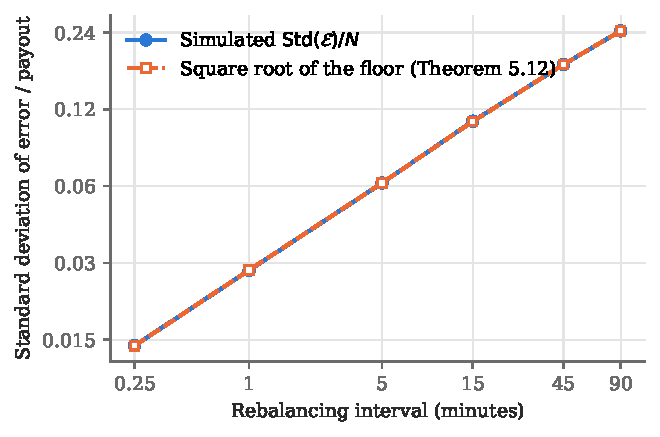
\includegraphics[width=0.7\textwidth]{figures/fig_frequency.pdf}
\caption{Standard deviation of the hedge error of the frictionless bilinear hedge as a function of the rebalancing interval, for $N=1{,}000$ (logarithmic scales). The simulated value and the square root of the variance floor of \cref{thm:pythagoras} coincide.}
\label{fig:frequency}
\end{figure}

\subsection{Frictions and band policies}

\Cref{fig:bands} shows the expected friction cost and the standard deviation of the error of band policies with half-widths $h^A = h^B = \eta N$, for a payout $N=10{,}000$. The bilinear hedge ($\eta=0$) costs $0.072N$ in expectation, of which $0.028N$ is the entry cost, and its error has standard deviation $0.041N$. In every case the mean error equals minus the expected friction cost to within sampling error, as \cref{prop:decomposition-frictions} predicts. Narrow bands ($\eta\leq 0.02$) reduce the friction cost by up to $10\%$ without increasing the standard deviation; for $\eta=0.01$ it is even slightly lower, because suppressing small trades also removes part of the randomness of the friction cost, as allowed by \eqref{eq:std-bound}. Wider bands keep reducing the friction cost, to $0.015N$ for $\eta=0.4$, but the standard deviation then grows quickly, to $0.22N$, within the bound of \cref{prop:band}(b).

\begin{figure}[ht]
\centering
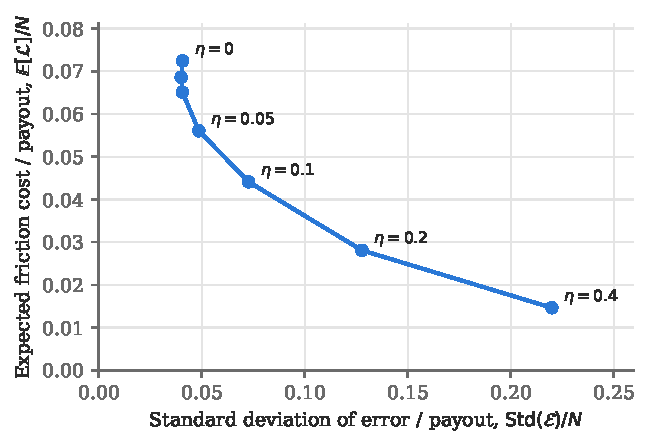
\includegraphics[width=0.7\textwidth]{figures/fig_bands.pdf}
\caption{Expected friction cost against standard deviation of the hedge error for band policies with half-widths $\eta N$, for $N=10{,}000$ and rebalancing every minute. The unlabelled points between $\eta=0$ and $\eta=0.05$ are $\eta=0.01$ and $\eta=0.02$.}
\label{fig:bands}
\end{figure}

The simulation also illustrates the crossed-liquidity property of \cref{sec:frictions}. The book of $A$ is wide $8.1\%$ of the time, and $8.2\%$ of the rebalancing volume in $A$ (excluding the entry trade) is traded while it is wide. The hedge of $A$ is triggered by goals in match $B$, so its trades are essentially unrelated to the state of the book of $A$: they meet a wide book only as often as a randomly timed trade would. A hedge whose trades in $A$ were triggered by goals in match $A$ would instead trade systematically in the minutes when that book is widest.

\subsection{Quoted odds}

Finally, we compute the quoted odd of \cref{thm:odd} with margin $m=0.05$ and risk tolerance $\lambda\in\{0.25,1\}$. For a grid of payouts from $100$ to $80{,}000$, the friction premium $R_\lambda(N)$ is minimised over band policies with $\eta\in\{0,0.01,0.02,0.05,0.1,0.2,0.4\}$, the effective price $g$ is interpolated linearly in $\log N$, and the fixed point \eqref{eq:fixed-point} is solved by bisection. On this grid, the effective price is non-decreasing for both values of $\lambda$, so \cref{ass:regular} holds.

\Cref{fig:odds} shows the result. The competitive odd $(1-m)/(p_Ap_B)$ is $4.96$. The static superhedge supports an odd of only $2.35$ for small stakes, falling to $1.78$ for a stake of $20{,}000$. The dynamic hedge supports $3.76$ for small stakes with $\lambda=1$ and $4.16$ with $\lambda=0.25$, falling to $2.31$ and $3.14$ respectively at a stake of $20{,}000$. For small payouts, the premium over $p_Ap_B$ splits roughly equally between the expected friction cost, mostly spread, and the risk charge, mostly the variance floor: at $N=500$ with $\eta=0.01$, both $\E[\mathcal{L}]/N$ and $\operatorname{Std}(\mathcal{E})/N$ are about $0.03$. For large payouts, impact dominates, and the optimal band widens: with $\lambda=1$, the optimal $\eta$ rises from $0.01$ for $N\leq 2{,}000$ to $0.2$ for $N\geq 40{,}000$. With $\lambda=0.25$, the optimal $\eta$ reaches the edge of the grid ($0.4$) for the largest payouts, so the odds shown for the largest stakes slightly understate what a finer search would give.

\begin{figure}[ht]
\centering
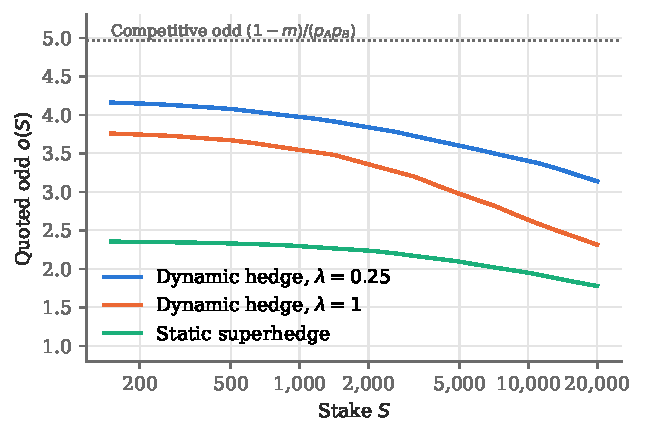
\includegraphics[width=0.7\textwidth]{figures/fig_odds.pdf}
\caption{Quoted odd as a function of the stake (logarithmic scale), with margin $m=0.05$, for the dynamic hedge with two risk tolerances and for the static superhedge. The dotted line is the competitive odd.}
\label{fig:odds}
\end{figure}

The dynamic hedge thus closes a substantial part of the gap between the static and the competitive odd, more so for small stakes and lower risk aversion. In this calibration, the remaining gap at small stakes comes from two sources that a bookmaker can address: the variance floor, which falls with more frequent rebalancing (\cref{fig:frequency}) and diversifies across a portfolio of parlays (\cref{sec:robust}), which supports a lower effective $\lambda$ per bet; and the spread, which falls with passive execution.

% ==================================================================
\section{Conclusion}
\label{sec:conclusion}
% ==================================================================
We studied how a bookmaker without a view on outcomes can quote a parlay using only the order books of a prediction market on the individual legs. For a single event, buying the payout in contracts is an exact, static hedge, and the resulting odd is the market's own price net of margin. For a parlay on simultaneous events without a joint market, no such hedge exists. Every static hedge, and every dynamic hedge required to be safe on every path, costs at least the upper Fréchet bound: the bookmaker would quote the odd of the least likely leg alone, and a bettor would do better with single bets.

A competitive quote therefore requires two departures from the single-event case: trading while the events are live, and accepting a hedge error that is controlled on average rather than ruled out. Under the assumptions that fair values are martingales and that legs are conditionally independent, an exact product identity gives the variance-optimal hedge in closed form. Each leg is held in proportion to the fair value of the parlay on the other legs, so that a move in one leg is hedged by trading the others. Its residual error is the covariation of the legs' fair values, which is unhedgeable, measurable in real time, and vanishes as rebalancing becomes frequent unless the legs move together. The analysis also clarifies what hedging does: the mean of the error is set by the capital charged, whatever the strategy, while the strategy determines the dispersion and, with order books, the friction cost.

With order books, the hedging cost splits into the market-implied premium and a risk-adjusted friction premium, which the bookmaker minimises over policies such as no-trade bands. The quoted odd solves a fixed-point equation of the same form as the single-event odd, with an effective price per unit of payout in place of the average execution price. It lies between the static odd and the competitive parlay odd, approaching the latter when books are deep and legs independent. In a simulation of two football matches, the dynamic hedge closes much of the gap between the two.

Several questions remain open. The acceptance criterion based on the standard deviation is convenient but penalises gains and is not monotone; downside criteria such as a limit on conditional value at risk would be more natural, at the cost of the closed-form results. The treatment of dependent legs, in particular within the same game, requires models of joint dynamics that we have only sketched. Execution with passive orders, adverse selection by informed bettors, and the management of a portfolio of parlays sharing legs are important in practice and would each deserve a study of their own. Finally, calibrating the model on historical order-book data from live prediction markets would show how much of the theoretical gain survives in real markets.

\begin{thebibliography}{99}

\bibitem{DavisPanasZariphopoulou1993}
M.~H.~A. Davis, V.~G. Panas, and T.~Zariphopoulou.
\newblock European option pricing with transaction costs.
\newblock \emph{SIAM Journal on Control and Optimization}, 31(2):470--493, 1993.

\bibitem{FollmerSchweizer1991}
H.~Föllmer and M.~Schweizer.
\newblock Hedging of contingent claims under incomplete information.
\newblock In M.~H.~A. Davis and R.~J. Elliott, editors, \emph{Applied Stochastic Analysis}, volume~5 of \emph{Stochastics Monographs}, pages 389--414. Gordon and Breach, London, 1991.

\bibitem{Frechet1951}
M.~Fréchet.
\newblock Sur les tableaux de corrélation dont les marges sont données.
\newblock \emph{Annales de l'Université de Lyon, Section A}, 14:53--77, 1951.

\bibitem{KarlisNtzoufras2009}
D.~Karlis and I.~Ntzoufras.
\newblock Bayesian modelling of football outcomes: using the Skellam's distribution for the goal difference.
\newblock \emph{IMA Journal of Management Mathematics}, 20(2):133--145, 2009.

\bibitem{KunitaWatanabe1967}
H.~Kunita and S.~Watanabe.
\newblock On square integrable martingales.
\newblock \emph{Nagoya Mathematical Journal}, 30:209--245, 1967.

\bibitem{Maher1982}
M.~J. Maher.
\newblock Modelling association football scores.
\newblock \emph{Statistica Neerlandica}, 36(3):109--118, 1982.

\bibitem{Rockafellar1970}
R.~T. Rockafellar.
\newblock \emph{Convex Analysis}.
\newblock Princeton University Press, Princeton, NJ, 1970.

\bibitem{Schweizer1995}
M.~Schweizer.
\newblock Variance-optimal hedging in discrete time.
\newblock \emph{Mathematics of Operations Research}, 20(1):1--32, 1995.

\bibitem{Skellam1946}
J.~G. Skellam.
\newblock The frequency distribution of the difference between two Poisson variates belonging to different populations.
\newblock \emph{Journal of the Royal Statistical Society}, 109(3):296, 1946.

\bibitem{SonerShreveCvitanic1995}
H.~M. Soner, S.~E. Shreve, and J.~Cvitanić.
\newblock There is no nontrivial hedging portfolio for option pricing with transaction costs.
\newblock \emph{The Annals of Applied Probability}, 5(2):327--355, 1995.

\bibitem{WhalleyWilmott1997}
A.~E. Whalley and P.~Wilmott.
\newblock An asymptotic analysis of an optimal hedging model for option pricing with transaction costs.
\newblock \emph{Mathematical Finance}, 7(3):307--324, 1997.

\bibitem{WolfersZitzewitz2004}
J.~Wolfers and E.~Zitzewitz.
\newblock Prediction markets.
\newblock \emph{Journal of Economic Perspectives}, 18(2):107--126, 2004.

\end{thebibliography}

\end{document}
